\chapter{Proof Repair by Example}

The first tool (PUMPKIN PATCH) focuses on changes in programs and specifications, though these changes are limited in scope as we'll see later.

What this tool does is, when programs and specifications change and this breaks a lot of proofs, it lets the proof engineer fix just one of those proofs. It then generalizes the example patch into something that can fix other proofs broken by the same change.

So in other words, the information from those changes is carried in the difference between the old and new version of the example patched proof.
PUMPKIN PATCH generalizes that information.

Application can be automated in some cases at the end, or it can be manual.

The work saved is shown retroactively on case studies replaying changes from large proof devleopments in Git. Results for this tool are preliminary compared to what we'll see later, since this was the first prototype.

\section{Motivating Example}

PUMPKIN PATCH intro \& automation, reimagined

\section{Approach}

Parts of PUMPKIN PATCH Motivating the Core, plus more

Like I mentioned earlier, this works using differencing and program transformations. And of course all of this happens over proof terms.
Here's the system diagram.

Here, differencing thus looks at the difference between versions of the example patched proof for this information, and finds something called a patch candidate---which is localized to the context of the example, but not enough to fix other proofs broken by the change.

Then, program transformations generalize that candidate to a reusable proof patch, something that can fix other proofs broken by the same change.
Application works with hint databases or is manual.

\section{Differencing}

parts of PUMPKIN PATCH Inside the Core, Testing Boundaries, Future Work

How differencing works in detail

Limitations and whether they're addressed in later tools yet or not

\section{Transformation}

parts of PUMPKIN PATCH Inside the Core, Testing Boundaries, Future Work

How the four transformations work in detail

Limitations and whether they're addressed in later tools yet or not

\section{Implementation}

parts of PUMPKIN PATCH Inside the Core, plus more

\subsection{Tool Details}

\subsection{Workflow Integration}

\section{Results}

PUMPKIN PATCH Case Studies, key technical results

\section{Conclusion}

Rehashing thesis and how we do it

What we haven't accomplished yet at this point (parts of PUMPKIN PATCH future work), segue into next chapter

% TODO for now, just a copy-paste of PUMPKIN PATCH original paper, including the bib---will change soon
% TODO program repair

%\section{Introduction}

%Proof assistants allow programmers to verify everything from distributed systems~\cite{wilcox:verdi} and compilers~\cite{leroy:compcert} to
%formalizations of mathematics~\cite{DBLP:journals/corr/BauerGLSSS16}. 

Proof automation makes verification more accessible to programmers, but it is often intractable
without programmer guidance. In \textit{interactive theorem proving} (ITP), the programmer guides the 
proof search process. The guidance reduces the search space to make proof automation more tractable.
This in turns helps the programmer, who does not have to manually verify the entire system.

%Interactive theorem provers allow programmers to guide proof search and interactively 
%verify everything from distributed systems~\cite{wilcox:verdi} and compilers~\cite{leroy:compcert} to
%formalizations of mathematics~\cite{DBLP:journals/corr/BauerGLSSS16}. In many of these theorem provers, programmers use

%In these languages, programmers write precise specifications of programs
%and prove implementations correct with respect to the specifications.

Despite automation, programming in these proof assistants is brittle: Even a minor change to a definition or theorem
can break many dependent proofs. This is a major source of development inefficiency in proof assistants
based on dependent type theory~\cite{proof-eng, Aydemir2008, Delaware2013ICFP}.

Traditional proof automation does not consider how proofs, definitions, and theorems change over time.
Instead, it is driven by the state of the current proof, sometimes with supplementary
information from other proofs, definitions, and theorems (as in hint databases~\cite{hints} and rippling~\cite{rippling}).
This puts the burden of dealing with brittleness on the programmer. 

We present a new approach to proof automation that accounts for breaking changes. %:
%searching the difference in versions of a proof, definition, or theorem. 
%We reimagine the problem of proof reuse~\cite{Boite2004, Mulhern06proofweaving} 
%in the context of traditional automation for ITP. 
In our approach, the programmer guides proof search 
by providing an \textit{example} of how to adapt proofs to changes in definitions or theorems.
A tool then generalizes the example adaptation into a \textit{reusable patch} that the programmer can use to fix
other broken proofs.

In doing so, we chart a path for a future %of ITP 
that moves the burden of brittleness
away from the programmer and into proof automation. 
Programmers typically address brittleness through design principles that make proofs
resilient to change~\cite{proof-eng, Aydemir2008, Delaware2013ICFP}, or through program-specific proof automation~\cite{chlipala:cpdt}.
These techniques, while useful, have limitations: 
Planning a verification effort around future change is challenging, and program-specific automation requires specialized knowledge.
The programmer's ability to anticipate likely changes determines the robustness of both techniques in
the face of change. %The robustness of both techniques in the face of change is determined by the programmer's ability to anticipate likely changes. 
Even then, many breaking changes are outside of the programmer's control. Updating proof assistant
versions, for example, can break proofs regardless of planning or automation~\cite{verdicommit}.

\begin{figure*}[ht]
\begin{minipage}{0.48\textwidth}
\centering
\lstset{language=coq, aboveskip=0pt, belowskip=0pt}
\lstinputlisting[firstline=1, lastline=3]{repair/izr.tex}
\lstinputlisting[backgroundcolor=\color{orange!35},firstline=4,lastline=5]{repair/izr.tex}
\lstinputlisting[firstline=6, lastline=6]{repair/izr.tex}
\end{minipage}
\hfill
\begin{minipage}{0.48\textwidth}
\centering
\lstset{language=coq, aboveskip=0pt, belowskip=0pt}
\lstinputlisting[firstline=8, lastline=10]{repair/izr.tex}
\lstinputlisting[backgroundcolor=\color{orange!35},firstline=11,lastline=12]{repair/izr.tex}
\lstinputlisting[firstline=13, lastline=13]{repair/izr.tex}
\end{minipage}
\vspace{-.3cm}
%\setlength{\belowcaptionskip}{-2pt}
\caption[Caption]{Old (left) and new (right) definitions of \lstinline{IZR} in Coq.
The old definition applies injection from naturals to reals and conversion of positives to
naturals; the new definition applies injection from positives to reals.}
\label{fig:izr}
\end{figure*}


We identify a set of core components that are critical to searching an example for patches in Coq.
We use the components to build %four different 
a procedure for finding patches %for non-structural changes 
in a Coq plugin as a 
proof-of-concept.
Case studies on real projects like CompCert~\cite{leroy:compcert} and the Coq standard library
suggest that patches are useful for realistic scenarios, and that it is simple to compose the components 
to handle different classes of changes.
We test the boundaries of the components on a suite of tests
and show how our findings can help build the future we envision.

In summary, we contribute the following:

\begin{enumerate}
%\item We develop new foundations for proof automation in ITP that account for breaking changes. % TODO reword
\item We identify a set of core components that are key to searching for patches.
\item We demonstrate that these core components are useful on real changes in Coq code.
\item We explore how to drive a future that moves the burden of change in ITP away from the programmer and into automated tooling.
\end{enumerate}

% TODO fix contributions

% evaluation stuff in contributions too

% SOMEWHERE: we focus on non-structural changes





%\section{Automation, Reimagined}

Traditional proof automation considers only the current state of
theorems, proofs, and definitions. This is a missed opportunity: Verification projects 
are rarely static. Like other software, these projects evolve over time.

Currently, the burden of change largely falls on programmers.
This does not have to be true. Proof automation
can view theorems, proofs, and definitions as fluid entities:
When a proof or specification changes,
a tool can search the difference between the old and new versions
for a \emph{reusable patch} that can fix broken proofs.

\paragraph{Status Quo} Experienced Coq programmers use design principles and custom tactics to make proofs
resilient to change. These techniques are useful for large proof developments, but they 
%require expertise. Even then, they 
place the burden of change on the programmer. This can be problematic
when change occurs outside of the programmer's control. % How to ward off Adam Chlipala here?

Consider a commit from the upcoming Coq 8.7 release~\cite{coq87commit}. 
This commit redefined injection from integers to reals (Figure~\ref{fig:izr}).
This change broke 18 proofs in the standard library. 

The Coq developer who committed the change fixed the broken proofs, then
made an additional 12 commits to address the change in \lstinline{coq-contribs},
a regression suite of projects that the Coq developers maintain as versions change.
Many of these changes were simple. For example, the developer wrote a lemma that describes the change:

\lstset{language=coq, aboveskip=3pt, belowskip=3pt}
\begin{lstlisting}
    Lemma INR_IPR : (@\ltacforall@)p, INR (Pos.to_nat p) = IPR p.
\end{lstlisting}

The developer then used this lemma to fix broken proofs within the standard library. 
For example, one proof broke on this line:

\begin{lstlisting}
    (@\fails{rewrite Pos2Nat.inj\_sub by trivial.}@)
\end{lstlisting}

It succeeded with the lemma:

\begin{lstlisting}
    rewrite (@\diff{<- 3!INR\_IPR}@), (@\succeeds{Pos2Nat.inj\_sub by trivial.}@)
\end{lstlisting}

These changes are outside-facing: Coq users have to make similar changes to their own proofs when
they update to Coq 8.7. The Coq developer can update some tactics to account for this, but it is 
impossible to account for every tactic that users could use.
Furthermore, while the developer responsible for the changes knows about
the lemma that describes the change, the Coq user does not. The Coq user must determine
how the definition has changed and how to address the change, perhaps by reading documentation or by
talking to the developers. 

\paragraph{Our Vision} When a user updates Coq, a tool can determine
that the definition has changed, then analyze changes in the standard library and in \lstinline{coq-contribs}
that resulted from the change in definition (in this case, rewriting by the lemma).
It can extract a reusable patch from those changes, which it can automatically apply within broken user proofs.
The user never has to consider how the definition has changed.

% TODO talk about the search space

% This isn't an example we actually handle yet, but I think that's OK for this section
% Mostly just had dependency issues trying to pull this code and so on, since I'm no on 8.7
% But it's topical and outside-facing


%\section{Generating Reusable Patches}
\label{sec:sys}

We identify five components that are key to finding reusable patches.
We implement these components in a prototype Coq plugin, which we call
\sysnamelong (Proof Updater Mechanically Passing Knowledge Into New Proofs, Assisting The Coq Hacker), or \sysname.\footnote{\url{http://github.com/uwplse/PUMPKIN-PATCH/tree/cpp18}}

We focus the \sysname prototype on the proof assistant Coq~\cite{coq}.
In Coq, each theorem is a type, and a proof of that theorem is a term that inhabits that type. 
Rather than write proof terms directly, users write proof scripts in a high-level tactic language;
Coq then uses these scripts to guide search for a proof term.
%We discuss supporting other proof assistants in Section~\ref{sec:future}.

The \sysname repository contains 
a detailed user guide.
To use \sysname, the programmer modifies a single proof script to provide an \textit{example} of how to adapt a proof to a
change. \sysname generalizes the example adaptation into a \textit{reusable patch}: a function
that can be used to fix other broken proofs, which \sysname defines as a Coq term.
We focus on the problem of \textit{finding} these patches;
we discuss how to extend \sysname to automatically \textit{apply} patches it finds in Section~\ref{sec:future}.

We motivate the core components (Section~\ref{sec:coreintro}) and describe how they
compose to find patches (Section~\ref{sec:composeintro}). We find patches for 
real code in Section~\ref{sec:case}, and we describe our implementation
in Section~\ref{sec:core}.

\begin{figure*}[ht]
\begin{minipage}{0.50\textwidth}
\lstset{language=coq, aboveskip=0pt, belowskip=0pt}
\lstinputlisting[firstline=1, lastline=1]{repair/introex.tex}
\lstinputlisting[backgroundcolor=\color{orange!35},firstline=2,lastline=2]{repair/introex.tex}
\lstinputlisting[firstline=3, lastline=8]{repair/introex.tex}
\lstinputlisting[firstline=1, lastline=4]{repair/introexterm.tex}
\lstinputlisting[backgroundcolor=\color{orange!35},firstline=5,lastline=5]{repair/introexterm.tex}
\lstinputlisting[firstline=6, lastline=9]{repair/introexterm.tex}
\end{minipage}
\hfill
\begin{minipage}{0.48\textwidth}
\lstset{language=coq, aboveskip=0pt, belowskip=0pt}
\lstinputlisting[firstline=9, lastline=9]{repair/introex.tex}
\lstinputlisting[backgroundcolor=\color{orange!35},firstline=10,lastline=10]{repair/introex.tex}
\lstinputlisting[firstline=11, lastline=16]{repair/introex.tex}
\lstinputlisting[firstline=11, lastline=14]{repair/introexterm.tex}
\lstinputlisting[backgroundcolor=\color{orange!35},firstline=15,lastline=15]{repair/introexterm.tex}
\lstinputlisting[firstline=16, lastline=19]{repair/introexterm.tex}
\end{minipage}
\vspace{-.4cm}
\setlength{\belowcaptionskip}{-4pt}
\caption{Two proofs with different conclusions (top) and the
corresponding proof terms (bottom) with relevant type information. We highlight the change in theorem conclusion and
the difference in terms that corresponds to a patch.}
\label{fig:example}
\end{figure*}

\subsection{Motivating the Core}
\label{sec:coreintro}

We identify and isolate
five core components critical to finding reusable patches:

\begin{enumerate}
\item \textit{Semantic differencing} between terms
\item \textit{Patch specialization} to arguments
\item \textit{Patch abstraction} of arguments or functions
\item \textit{Patch inversion} to reverse a patch
\item \textit{Lemma factoring} to break a term into parts
\end{enumerate}

The semantic differencing component finds the difference between two terms, which produces a \textit{candidate} for
a reusable patch. %However, this candidate may not be the final patch the tool is looking for.
 %: It may be too general or too specific,
%for example. 
The other components modify the candidate to try to produce a patch.
To motivate this workflow, consider using \sysname to search the proofs in
Figure~\ref{fig:example} for a patch between conclusions. We invoke the plugin using \lstinline{old} and \lstinline{new}
as the example change:

\begin{lstlisting}[language=ml4]
    Patch Proof old new as patch.
\end{lstlisting}

\sysname first determines the type that a patch from \lstinline{new} to \lstinline{old} should have.
To determine this, it semantically \textit{diffs} the types and finds this goal type (line 2):

\begin{lstlisting}[language=coq]
    (@\ltacforall@) n m p, n <= m -> m <= p -> (@\diff{n <= p}@) -> (@\diff{n <= p + 1}@)
\end{lstlisting}

It then breaks each inductive proof into cases and determines an intermediate goal type for the candidate.
%recursively searches each case for a candidate.
In the base case, for example, it \textit{diffs} the types and determines that a candidate
between the base cases of \lstinline{new} and \lstinline{old} should have this type (lines 11 and 12):

\begin{lstlisting}
    (@\diff{(fun p0 => n <= p0)}@) m -> (@\diff{(fun p0 => n <= p0 + 1)}@) m
\end{lstlisting}

It then \textit{diffs} the terms (line 13) for such a candidate:

\begin{lstlisting}
    fun n m p H0 H1 =>(@\vspace{-0.04cm}@)
      (fun (H : n <= m) => (@\diff{le\_plus\_trans n m 1}@) H)(@\vspace{-0.04cm}@)
    : (@\ltacforall@) n m p, n <= m -> m <= p -> (@\diff{n <= m}@) -> (@\diff{n <= m + 1}@)
\end{lstlisting}

This candidate is close, but it is not yet a patch. This candidate
maps base case to base case (it is applied to \lstinline{m}); the patch should map conclusion to conclusion (it should
be applied to \lstinline{p}).
\sysname \textit{abstracts} this candidate by \lstinline{m} (line 11), which lifts it out of the base case:

\begin{lstlisting}
    fun (@\diff{n0}@) n m p H0 H1 =>(@\vspace{-0.04cm}@)
      (fun (H : n <= (@\diff{n0}@)) => le_plus_trans n (@\diff{n0}@) 1 H)(@\vspace{-0.04cm}@)
    : (@\ltacforall@) (@\diff{n0}@) n m p, n <= m -> m <= p -> n <= (@\diff{n0}@) -> n <= (@\diff{n0}@) + 1
\end{lstlisting}

%This produces a candidate that is closer: It is not yet a patch, but applying it to \lstinline{p} (line 16),
%the argument to the conclusion of \lstinline{le_ind}, will produce a patch.
\sysname then \textit{specializes} this candidate to \lstinline{p} (line 16), the argument
to the conclusion of \lstinline{le_ind}. This produces a patch:

\begin{lstlisting}
    patch n m p H0 H1 := (@\vspace{-0.04cm}@)
      (fun (H : n <= (@\diff{p}@)) => le_plus_trans n (@\diff{p}@) 1 H)(@\vspace{-0.04cm}@)
    : (@\ltacforall@) n m p, n <= m -> m <= p -> n <= (@\diff{p}@) -> n <= (@\diff{p}@) + 1
\end{lstlisting}

The user can then use \lstinline{patch} to fix other broken proofs.
For example, given a proof that applies \lstinline{old}, the user can use \lstinline{patch} to prove the same conclusion
by applying \lstinline{new}:

\begin{lstlisting}[language=coq]
    (@\succeeds{apply old.}@)(@\vspace{-0.1cm}@)
    (@\diff{apply patch.}@) (@\succeeds{apply new.}@)
\end{lstlisting}

This simple example uses only three components. The other components help turn candidates
into patches in similar ways. We discuss all five components in more detail in the
rest of this section.

\paragraph{Semantic Differencing} The tool should be able to identify the semantic difference between terms.
The semantic difference is the difference between two terms that corresponds to
the difference between their types. Consider the base case terms in Figure~\ref{fig:example} (line 13):

\begin{lstlisting}[language=coq]
    (@\diff{le\_plus\_trans n m 1}@) H : (@\diff{n <= m + 1}@)(@\vspace{-0.1cm}@)
    (@\phantom{le\_plus\_trans n m 1}@) H : (@\diff{n <= m}@)
\end{lstlisting}

The semantic differencing component first identifies the difference in their types, or the \textit{goal type}:

\begin{lstlisting}
    (@\diff{n <= m}@) -> (@\diff{n <= m + 1}@)
\end{lstlisting}

It then finds a difference in terms that has that type:

\begin{lstlisting}[language=coq]
    fun (H : n <= m) => (@\diff{le\_plus\_trans n m 1}@) H
\end{lstlisting}

%This is the core of any patching procedure: The terms that it finds are candidates for reusable patches.
%The other components modify these candidates to find true patches.
 % (for example, in this case, the abstraction component  may generalize this function to work with nu

% TODO this erases type differencing stuff for fixpoints, but maybe that's OK
% Also, doesn't talk about zooming into functions and so on
This is the \emph{candidate} for a reusable patch that the other components modify to find a patch.

Differencing operates over terms and types. Differencing tactics
is insufficient, since tactics and hints may mask patches
(line 5).\footnote{Since this is a simple example, replaying an existing tactic happens to work. There
are additional examples in the repository (\lstinline{Cex.v}).}
Furthermore, differencing is aware of the semantics of terms and types.
Simply exploring the syntactic difference %between terms 
makes it hard to identify
which changes are meaningful.
For example, in the inductive case (line 14), the inductive hypothesis
changes:

\begin{lstlisting}[language=coq]
    ... (IHle : (@\diff{n <= m0 + 1}@)) ...(@\vspace{-0.08cm}@)
    ... (IHle : (@\diff{n <= m0}@)) ...
\end{lstlisting}

However, the type of \lstinline{IHle} changes for \emph{any} two inductive proofs over \lstinline{le}
with different conclusions. A syntactic differencing component 
may identify this change as a candidate.
Our semantic differencing component knows that it can ignore this change.

\paragraph{Patch Specialization} The tool should be able to specialize a patch candidate to specific arguments as determined by
the differences in terms. To find a patch for Figure~\ref{fig:example}, for example, \sysname
must specialize the patch candidate to \lstinline{p} to produce the final patch.

%Consider searching two proofs of theorems with hypotheses for a patch between conclusions:

%\begin{lstlisting}[language=coq]
 %   (@\ltacforall@) n m p, n <= m -> m <= p -> n <= p + 1
  %  (@\ltacforall@) n m p, n <= m -> m <= p -> n <= p
%\end{lstlisting}

%Semantic differencing determines the goal type:

%\begin{lstlisting}[language=coq]
 %   (@\ltacforall@) n m p, n <= m -> m <= p -> n <= p -> n <= p + 1
%\end{lstlisting}

%A patch of this type may not show up explicitly in the difference of terms.
%The tool may instead find an abstract patch candidate:

%\begin{lstlisting}[language=coq]
 %   fun n m p H0 H1 =>
  %    (fun (@\diff{n0}@) (H : n <= (@\diff{n0}@)) => le_plus_trans n (@\diff{n0}@) 1 H)
   % : (@\ltacforall@) n m p (@\diff{n0}@),
   %   n <= m -> m <= p -> n <= (@\diff{n0}@) -> n <= (@\diff{n0}@) + 1
%\end{lstlisting}

%This does not quite have the correct type, but it \emph{does} have the correct type
%if we specialize it to \lstinline{p}:

%\begin{lstlisting}[language=coq]
 %   fun n m p H0 H1 =>
  %    (fun (H : n <= (@\diff{p}@)) => le_plus_trans n (@\diff{p}@) 1 H)
   % : (@\ltacforall@) n m p,
    %  n <= m -> m <= p -> n <= (@\diff{p}@) -> n <= (@\diff{p}@) + 1
%\end{lstlisting}

\paragraph{Patch Abstraction} A tool should be able to abstract patch candidates of this form by the common argument:

\begin{lstlisting}[language=coq]
    candidate : P' t -> P t(@\vspace{-0.08cm}@)
    candidate_abs : (@\ltacforall@) (@\diff{t0}@), P' (@\diff{t0}@) -> P (@\diff{t0}@)
\end{lstlisting}
and it should be able to abstract patch candidates of this form by the common function:

\begin{lstlisting}[language=coq]
    candidate : P t' -> P t(@\vspace{-0.08cm}@)
    candidate_abs : (@\ltacforall@) (@\diff{P0}@), (@\diff{P0}@) t' -> (@\diff{P0}@) t
\end{lstlisting} 

This is necessary because the tool may find candidates in an applied form.
For example, when searching for a patch between the proofs in Figure~\ref{fig:example},
\sysname finds a candidate in the difference of base cases. To produce a patch, 
\sysname must abstract the candidate by the argument \lstinline{m}.
Abstracting candidates is not always possible; abstraction will necessarily be a collection of heuristics.

\paragraph{Patch Inversion} The tool should be able to invert a patch candidate.
This is necessary to search for isomorphisms. %in both directions (that is, to find isomorphisms) between propositionally equal types.
It is also necessary to search for implications between propositionally
equal types, since candidates may appear in the wrong direction.
For example, consider two list lemmas (we write \lstinline{length} as \lstinline{len}):

\begin{lstlisting}[language=coq]
    old : (@\ltacforall@) l' l, len (l' ++ l) = len l' + len l(@\vspace{-0.08cm}@)
    new : (@\ltacforall@) l' l, len (l' ++ l) = len l' + len (rev l)
\end{lstlisting} 

If \sysname searches the difference in proofs of these lemmas for a patch from the 
conclusion of \lstinline{new} to the conclusion of \lstinline{old},
it may find a candidate \emph{backwards}: %, as a patch from \lstinline{old} to \lstinline{new}:

\begin{lstlisting}
    candidate l' l (H : (@\diff{old}@) l' l) :=(@\vspace{-0.04cm}@)
      eq_ind_r ... (@\diff{(rev\_length l)}@)(@\vspace{-0.04cm}@)
   : (@\ltacforall@) l' l, (@\diff{old}@) l' l -> (@\diff{new}@) l' l
\end{lstlisting}

The component can invert this to get the patch: %from \lstinline{new} to \lstinline{old}:

\begin{lstlisting}
    patch l' l (H : (@\diff{new}@) l' l) :=(@\vspace{-0.04cm}@)
      eq_ind_r ... (@\diff{(eq\_sym (rev\_length l))}@)(@\vspace{-0.04cm}@)
   : (@\ltacforall@) l' l, (@\diff{new}@) l' l -> (@\diff{old}@) l' l
\end{lstlisting}

We can then use this patch to port proofs.
For example, if we add this patch to a hint database~\cite{hints},
we can port this proof:

\begin{lstlisting}
    Theorem app_rev_len : (@\ltacforall@) l l',(@\vspace{-0.04cm}@)
      len (rev (l' ++ l)) = len (rev l) + len (rev l').(@\vspace{-0.04cm}@)
    Proof.(@\vspace{-0.04cm}@)
      intros. rewrite rev_app_distr. (@\succeeds{apply old.}@)
\end{lstlisting}
to this proof:

\begin{lstlisting}
      intros. rewrite rev_app_distr. (@\succeeds{apply new.}@)
\end{lstlisting}

Rewrites like \lstinline{candidate} are \textit{invertible}:
We can invert any rewrite in one direction by rewriting in the opposite direction.
In contrast, it is not possible to invert the patch \sysname
found for Figure~\ref{fig:example}.
Inversion will necessarily sometimes fail, since not all terms are invertible.
%Not all terms are invertible. It is not possible, for example, to invert the patch 
%Inversion will necessarily sometimes fail.

\paragraph{Lemma Factoring} The tool should be able to factor a term into a sequence of lemmas.
This can help break other problems, like abstraction, into smaller subproblems.
It is also necessary to invert certain terms.
Consider inverting an arbitrary sequence of two rewrites:

\begin{lstlisting}
    t := (@\diff{eq\_ind\_r G ...}@) ((@\diff{eq\_ind\_r F ...}@))
\end{lstlisting}

We can view \lstinline{t} as a term that composes two functions:

\begin{lstlisting}
    g := (@\diff{eq\_ind\_r G ...}@)(@\vspace{-0.04cm}@)
    f := (@\diff{eq\_ind\_r F ...}@)(@\vspace{-0.04cm}@)
    t := g $\circ$ f
\end{lstlisting}

The inverse of \lstinline{t} is the following:

\begin{lstlisting}
    t$\inv$ := f$\inv$ $\circ$ g$\inv$
\end{lstlisting}

To invert \lstinline{t}, \sysname identifies the factors \lstinline{[f; g]}, 
inverts each factor to \lstinline{[f}$\inv$\lstinline{; g}$\inv$\lstinline{]}, 
then folds and applies the inverse factors in the opposite direction.

\subsection{Composing Components}
\label{sec:composeintro}

% Note about tactics?

The components come together to form a proof patch finding procedure:

\begin{algorithm}
\begin{algorithmic}[1]
\renewcommand{\thealgorithm}{}
\footnotesize
\caption{\footnotesize{find\_patch(term, term', direction)}}
    \STATE \diff{\textit{diff} types of term and term' for goals}
    \STATE \diff{\textit{diff} term and term' for candidates}
    \IF{there are candidates}
      \STATE \diff{\textit{factor}, \textit{abstract}, \textit{specialize}, and/or \textit{invert} candidates}
      \IFRETURN{there are patches}{patches}
    \ENDIF
    \IF{direction is forwards}
      \STATE find\_patch(term', term, backwards) for candidates
      \STATE \textit{factor} and \textit{invert} candidates
      \IFRETURN{there are patches}{patches}
    \ENDIF
    \RETURN failure
\end{algorithmic}
\label{alg:patching}	
\end{algorithm}

\begin{figure*}[ht]
\begin{minipage}{0.48\textwidth}
\lstset{language=coq, aboveskip=0pt,belowskip=0pt}
\lstinputlisting[firstline=1, lastline=1]{repair/compcert.tex}
\lstinputlisting[backgroundcolor=\color{orange!35},firstline=2,lastline=2]{repair/compcert.tex}
\end{minipage}
\hfill
\begin{minipage}{0.48\textwidth}
\lstset{language=coq, aboveskip=0pt,belowskip=0pt}
\lstinputlisting[firstline=4, lastline=4]{repair/compcert.tex}
\lstinputlisting[backgroundcolor=\color{orange!35},firstline=5,lastline=5]{repair/compcert.tex}
\end{minipage}
\vspace{-.3cm}
%\setlength{\belowcaptionskip}{-4pt}
\caption[Caption for LOF]{Old (left) and new (right) definitions of \lstinline{int} in CompCert.}
\label{fig:int}
\end{figure*}

\sysname infers a \textit{configuration} from the example change.
This configuration customizes the highlighted lines for an entire class of changes:
It determines what to diff on lines 1 and 2,
and how to use the components on line 4.

For example, to find a patch for Figure~\ref{fig:example},
\sysname used the configuration for changes in conclusions of two proofs
that induct over the same hypothesis. Given two such
proofs:

%We describe one
%such procedure in this section; we descibe three more
%in Section~\ref{sec:case}.
\begin{lstlisting}[language=coq]
    (@\ltacforall@) x, H x -> (@\diff{P}@) x(@\vspace{-0.1cm}@)
    (@\ltacforall@) x, H x -> (@\diff{P'}@) x
\end{lstlisting}
\sysname searches for a patch with this type:

\begin{lstlisting}[language=coq]
    (@\ltacforall@) x, H x -> (@\diff{P'}@) x -> (@\diff{P}@) x
\end{lstlisting}
using this configuration:

\begin{algorithm}
\footnotesize
\begin{algorithmic}[1]
%  Is it really necessary to say that an algorithm might do initialization?
%  \STATE Build trees for search
  %\STATE build trees for proofs
  %\REPEAT
    \STATE \textit{diff} conclusion types for goals
    \STATE \textit{diff} conclusion terms for candidates
    \STATE \textbf{if} there are candidates \textbf{then}
    \STATE \hspace*{1em} \textit{abstract} and then \textit{specialize} candidates
\end{algorithmic}
\end{algorithm}

Section~\ref{sec:case} describes real-world examples that demonstrate more configurations.

%Scenarios from real-world examples in Section~\ref{sec:case} demonstrate more configurations.
%We discuss more configurations in Section~\ref{sec:case},
%and we describe our implementation in Section~\ref{sec:core}.

%We show three more procedures
%in Section~\ref{sec:case}.

%The type of this term takes the conclusion of \lstinline{new} to the conclusion of \lstinline{old} (line 5):

%\begin{lstlisting}
%    n <= p -> n <= p + 1
%\end{lstlisting}

%TODO If both passes fail, the algorithm defaults to returning a function that always produces the old term.





%\section{Case Studies: Changes in the Wild}
\label{sec:case}

We used the \sysname prototype to emulate three motivating scenarios from real-world code:

\begin{enumerate}
\item \textbf{Updating definitions} within a project \\
(CompCert, Section~\ref{sec:compcert})
\item \textbf{Porting definitions} between libraries \\
(Software Foundations, Section~\ref{sec:foundations})
\item \textbf{Updating proof assistant versions} \\
(Coq Standard Library, Section~\ref{sec:coq})
\end{enumerate}

The code we chose for these scenarios demonstrated different classes of changes.
For each case, we describe how \sysname configures the procedure to use the core components for that class of changes.
Our experiences with these scenarios suggest that patches are useful and that the components 
are effective and flexible.

%For each scenario, we describe the experience using \sysname
%as well as the algorithm and the core components the scenario used.

%For each use case, %we identified how to adapt \sysname.
%In doing so, 
%we identified which core components were useful.
%In total, we used all five core components, and we did not need any new components.
%We identified useful extensions to two components:
%semantic search and patch abstraction.

% Also new ways to combine them, new and unforeseen uses to existing components
% Lemma detection is subcase of goal detection

%\vspace{-0.1cm}
\paragraph{Identifying Changes} We identified Git commits from popular Coq projects that
demonstrated each scenario.
These commits updated proofs in response to breaking changes. %that broke as a result of some change.
%which we could use as an example for \sysname.
We emulated each scenario as follows:

\begin{enumerate}
\item \textit{Replay} an example proof update for \sysname
\item \textit{Search} the example for a patch using \sysname
\item \textit{Apply} the patch to fix a different broken proof
\end{enumerate}

%In each use case, we built new algorithms from the core components of 
%\sysname. In doing so, we identified any extensions necessary to improve
%the core components to handle new uses cases.

Our goal was to simulate incremental use of a patch finding tool,
at the level of a small change or a commit that follows best practices.
We favored commits with changes that we could
isolate. When isolating examples for \sysname, we replayed changes from the bottom up,
as if we were making the changes ourselves.
This means that we did not always make the same change as the user. For example,
the real change from Section~\ref{sec:compcert} updated multiple definitions;
we updated only one.

\sysname is a proof-of-concept and does not yet handle some kinds of proofs.
In each scenario, we made minor modifications to proofs so that we could use \sysname (for example,
using induction instead of destruction).
\sysname does not yet handle structural changes like adding constructors or parameters, 
so we focused on changes that preserve shape, like modifying constructors.
We discuss supporting these features and whether they may necessitate other components in Section~\ref{sec:future}.
%Supporting these features is a matter of engineering, which we leave to future work 

\begin{figure*}[ht]
\begin{minipage}{0.48\textwidth}
\lstset{language=coq, aboveskip=0pt,belowskip=0pt} % blindFS / User A
\lstinputlisting[firstline=2, lastline=4]{repair/bintonat.tex}
\lstinputlisting[backgroundcolor=\color{orange!35},firstline=5,lastline=6]{repair/bintonat.tex}
\lstinputlisting[firstline=7, lastline=7]{repair/bintonat.tex}
\end{minipage}
\hfill
\begin{minipage}{0.48\textwidth}
\lstset{language=coq, aboveskip=0pt,belowskip=0pt}  % marshall / user B
\lstinputlisting[firstline=10, lastline=12]{repair/bintonat.tex}
\lstinputlisting[backgroundcolor=\color{orange!35},firstline=13,lastline=14]{repair/bintonat.tex}
\lstinputlisting[firstline=15, lastline=15]{repair/bintonat.tex}
\end{minipage}
\vspace{-.35cm}
%\setlength{\belowcaptionskip}{-4pt}
\caption[Caption for LOF]{Definitions of \lstinline{bin_to_nat} for Users A (left) and B (right).}
\label{fig:bintonat}
\end{figure*}

\lstset{language=coq, aboveskip=3pt,belowskip=3pt}

%\vspace{-0.1cm}
%\subsection{Patching Proofs\\\textit{\small{CompCert}}}
\subsection{Updating Definitions}
\label{sec:compcert}

Coq programmers sometimes make changes to definitions that break proofs
within the same project. To emulate this use case, 
we identified a CompCert commit~\cite{compcertcommit}
with a breaking change to \lstinline{int} (Figure~\ref{fig:int}). %The commit message notes that the new representation is more efficient.
We used \sysname to find a patch that corresponds to the change in \lstinline{int}.
The patch \sysname found fixed broken inductive proofs.

% TODO still need to ask Xavier, not sure if this depends on other definitions also changing


%to find a patch between versions of a changed constructor of an inductive type.
%This patched broken inductive proofs.
%In doing so, we used all five of the core components---four of them without any changes.

%\vspace{-0.1cm}
\paragraph{Replay} We used the proof of \lstinline{unsigned_range} as the example for \sysname.
The proof failed with the new \lstinline{int}:

\lstset{language=coq, aboveskip=3pt,belowskip=3pt}
\begin{lstlisting}[language=coq]
   Theorem unsigned_range:(@\vspace{-0.04cm}@)
     (@\ltacforall@)(i : int), 0 <= unsigned i < modulus.(@\vspace{-0.04cm}@)
   Proof.(@\vspace{-0.04cm}@)
     intros i. induction i using int_ind; auto(@\fails{.}@)
\end{lstlisting}

We replayed the change to \lstinline{unsigned_range}:

\begin{lstlisting}[language=coq]
     intros i. induction i using int_ind. (@\diff{simpl. omega}@)(@\succeeds{.}@)
\end{lstlisting}

%\vspace{-0.1cm}
\paragraph{Search} We used \sysname to search the example for a patch that corresponds to the change in \lstinline{int}. It found
a patch with this type:

\begin{lstlisting}[language=coq]
   (@\ltacforall@) z : Z,(@\vspace{-0.04cm}@) (@\diff{-1 < z < modulus}@) -> (@\diff{0 <= z < modulus}@)
\end{lstlisting}

%\vspace{-0.1cm}
\paragraph{Apply} After changing the definition of \lstinline{int}, the proof of the
theorem \lstinline{repr_unsigned} failed on the last tactic:

\begin{lstlisting}[language=coq]
   Theorem repr_unsigned:(@\vspace{-0.04cm}@)
     (@\ltacforall@)(i : int), repr (unsigned i) = i.(@\vspace{-0.04cm}@)
   Proof.(@\vspace{-0.04cm}@)
     ... apply Zmod_small; auto(@\fails{.}@)
\end{lstlisting}

Manually trying \lstinline{omega}---the tactic which helped us in the proof of \lstinline{unsigned_range}---did not
succeed.
We added the patch that \sysname found to a hint database.
The proof of the theorem \lstinline{repr_unsigned} then went through:

\begin{lstlisting}[language=coq]
    ... apply Zmod_small; auto(@\succeeds{.}@)
\end{lstlisting}

%\vspace{-0.1cm}
\subsubsection{Core Components}

%\paragraph{The Problem} The algorithm for changes in constructors of inductive
%types needed to produce patches with a form we had not yet encountered.
%The algorithm for changes in conclusions of proofs that induct over the same
%type produced patches with this form:

%\begin{lstlisting}[language=coq]
 %  (@\ltacforall@)(x : T), P x -> P' x
%\end{lstlisting}

This scenario used the configuration for changes in constructors of an inductive type.
Given such a change: %of an inductive type:

\begin{lstlisting}[language=coq]
   Inductive (@\diff{T}@) := ... | C : ... -> (@\diff{H}@) -> T(@\vspace{-0.08cm}@)
   Inductive (@\diff{T'}@) := ... | C : ... -> (@\diff{H'}@) -> T'
\end{lstlisting}
\sysname searches two inductive proofs of theorems:

\begin{lstlisting}[language=coq]
   (@\ltacforall@) (t : (@\diff{T}@)), P t(@\vspace{-0.08cm}@)
   (@\ltacforall@) (t : (@\diff{T'}@)), P t
\end{lstlisting}
for an isomorphism\footnote{If \sysname finds just one implication, it returns that.} between the constructors:

\begin{lstlisting}[language=coq]
   ... -> (@\diff{H}@) -> (@\diff{H'}@)(@\vspace{-0.1cm}@)
   ... -> (@\diff{H'}@) -> (@\diff{H}@)
\end{lstlisting}

The user can apply these patches within the inductive case that corresponds to the constructor \lstinline{C}
to fix other broken proofs that induct over the changed type. 
\sysname uses this configuration for changes in constructors:

\begin{algorithm}
\footnotesize
\begin{algorithmic}[1]
%  Is it really necessary to say that an algorithm might do initialization?
%  \STATE Build trees for search
  %\STATE build trees for proofs
  %\REPEAT
    \STATE \textit{diff} inductive constructors for goals
    \STATE use \textit{all components} to recursively search for changes in conclusions of the corresponding case of the proof
    \STATE \textbf{if} there are candidates \textbf{then}
    \STATE \hspace*{1em} try to \textit{invert} the patch to find an isomorphism 
\end{algorithmic}
\end{algorithm}

%We found it natural to use this patch within
%inductive proofs; if necessary, we can construct a patch that maps between types instead of constructors
%by applying the patch within the induction principle.
% TODO do we ever have to generalize by P? Why or why not?

%\paragraph{The Extension} It was simple to adapt \sysname to handle changes in the constructor of an inductive type. 
%We extended the type search algorithm to find search goals that correspond to changes in constructors.
%We used the other four components without any changes.

%\subsection{Porting Definitions\\\textit{\small{Software Foundations}}}

\subsection{Porting Definitions}
\label{sec:foundations}

Coq programmers sometimes port theorems and proofs to use definitions
from different libraries.
To simulate this, we used \sysname to port two solutions~\cite{usera, userb}
to an exercise in Software Foundations to each use the other solution's definition of the fixpoint \lstinline{bin_to_nat} (Figure~\ref{fig:bintonat}).
We demonstrate one direction; the opposite was similar.
%We used \sysname to find a patch between versions of a fixpoint;
%this patched inductive proofs about \lstinline{bin_to_nat}.
%We used \sysname to port User A's proofs to User B's definition and to port User B's proofs to User A's definition.

%In doing so, we used all five components---four without any changes.

%We also combined components in ways that we had not yet encountered,
%which may It combined components in ways that we had not yet encountered,
%which may help us improve our algorithms. It also demonstrated a new use case for abstraction
%that we had not considered; we were able to adapt \sysname to handle this easily.

% With this framing we lose the "why not tactics," but notably all of these are not obvious from tactics

%\vspace{-0.1cm}
\paragraph{Replay} We used the proof of \lstinline{bin_to_nat_pres_incr} from User A as the example for \sysname.
User A cut an inline lemma in an inductive case and proved it using a rewrite:

\begin{lstlisting}[language=coq]
   assert ((@\ltacforall@)a, S (a + S (@\diff{(a + 0)}@)) = S (S (a + (@\diff{(a + 0)}@)))).(@\vspace{-0.04cm}@)
   (@\ltacba@) ... (@\diff{rewrite <- plus\_n\_O.}@) rewrite -> plus_comm.
\end{lstlisting} % blindFS / user A

When we ported User A's solution to use User B's definition of \lstinline{bin_to_nat}, 
the application of this inline lemma failed. We changed the conclusion of the inline lemma 
and removed the corresponding rewrite:

\begin{lstlisting}[language=coq]
   assert ((@\ltacforall@)a, S (a + S a) = S (S (a + a))).(@\vspace{-0.04cm}@)
   (@\ltacba@) ... rewrite -> plus_comm.
\end{lstlisting} % blindFS / user A, adapted

%\vspace{-0.1cm}
\paragraph{Search} We used \sysname to search the example
for a patch that corresponds to the change in \lstinline{bin_to_nat}.
It found an isomorphism:

\begin{lstlisting}[language=coq]
   (@\ltacforall@)P b, P (@\diff{(bin\_to\_nat b)}@) -> P (@\diff{(bin\_to\_nat b + 0)}@)(@\vspace{-0.08cm}@)
   (@\ltacforall@)P b, P (@\diff{(bin\_to\_nat b + 0)}@) -> P (@\diff{(bin\_to\_nat b)}@)
\end{lstlisting}

%The only semantic difference between the two definitions of \lstinline{bin_to_nat} was that in 
%each recursive case,
%User A had one occurrence of \lstinline{bin_to_nat b' + 0} where User B had \lstinline{bin_to_nat b'}.

%This found an abstracted version of the term produced by the rewrite by \lstinline{plus_n_O},
%and inverted the abstract patch so that it can be used in both directions.

%\sysname was able to find a patch for this proof by searching the difference in proof terms of \lstinline{bin_to_nat_pres_incr}.
%In particular, each proof of \lstinline{bin_to_nat_pres_incr} passes through an inline lemma. \sysname found a patch
%between the conclusions of the inline lemmas, which had the type:

%\begin{lstlisting}[language=coq]
%   (@\ltacforall@)a,
%     S (a + S (@\remove{(}@)a (@\remove{+ 0)}@)) = S (S (a + (@\remove{(}@)a (@\remove{+ 0)}@))) ->
%     S (a + S (a + 0)) = S (S (a + (a + 0)))
%\end{lstlisting}

%In other words, for a specific property \lstinline{P}, this patch had the type:

%\begin{lstlisting}[language=coq]
 %  (@\ltacforall@)a, P a -> P (a + 0)
%\end{lstlisting}
%
%\sysname then applied that patch to the argument the lemma was applied to in each theorem:

%\begin{lstlisting}[language=coq]
%   (@\ltacforall@)b, P (bin_to_nat b) -> P (bin_to_nat b + 0)
%\end{lstlisting}

%\sysname then abstracted the result to work for any property:

%\begin{lstlisting}[language=coq]
%   (@\ltacforall@)P b, P (bin_to_nat b) -> P (bin_to_nat b + 0)
%\end{lstlisting}

%Finally, \sysname inverted the result to find the patch in the opposite direction:

%\begin{lstlisting}[language=coq]
%   (@\ltacforall@)P b, P (bin_to_nat b + 0) -> P (bin_to_nat b)
%\end{lstlisting}

%\vspace{-0.1cm}
\paragraph{Apply} After porting to User B's definition, a rewrite in the proof of the theorem
\lstinline{normalize_correctness} failed:

\begin{lstlisting}[language=coq]
   Theorem normalize_correctness:
     (@\ltacforall@)b, nat_to_bin (bin_to_nat b) = normalize b.
   Proof.
     ... (@\fails{rewrite -> plus\_0\_r.}@)
\end{lstlisting}

Attempting the obvious patch from the difference in tactics---rewriting by \lstinline{plus_n_O}---failed.
Applying the patch that \sysname found fixed the broken proof:

\begin{lstlisting}[language=coq]
     ... (@\diff{apply patch\_inv.}@) (@\succeeds{rewrite -> plus\_0\_r.}@)
\end{lstlisting}

% TODO shorten this:

In this case, since we ported User A's definition to a simpler 
definition,\footnote{User A uses \lstinline{*}; User B uses \lstinline{+}. 
For arbitrary \lstinline{n}, the term \lstinline{2 * n} reduces to \lstinline{n + (n + 0)}, which does not reduce any further.}
\sysname found a patch that was not the most natural patch.
The natural patch would be to remove the rewrite, just as we removed a different rewrite from the example proof.
This did not occur when we ported User B's definition,
which suggests that in the future, a patch finding tool may help inform novice users which definition is simpler:
It can factor the proof, %into a sequence of lemmas, 
then inform the user if two factors are inverses. %, who can remove the admissable tactics.
Tactic-level changes do not provide enough information to determine this; the tool must have a semantic
understanding of the terms.

%\paragraph{User A $\rightarrow$ User B}


%\paragraph{User B $\rightarrow$ User A}

%Porting in the opposite direction worked similarly. 
%User B proved \lstinline{bin_to_nat_pres_incr} through a more general auxiliary lemma:

%\begin{lstlisting}[language=coq]
 %  (@\ltacforall@)a b, S a + S b = S (S (a + b)).
%\end{lstlisting} % marshall / user B

%To port user B's proof, we added a rewrite by \lstinline{plus_n_O}. \sysname searched the difference of those auxiliary lemmas,
%applied the patch, and abstracted and inverted it accordingly.

%Both the patch and the inverse patch were useful for two later proofs. In both inductive cases
%of a lemma \lstinline{bin_to_nat_plus}, we were able to patch each broken line:

%\begin{lstlisting}[language=coq]
%   (@\fails{reflexivity.}@)
%\end{lstlisting}

%By applying the patch:

%\begin{lstlisting}[language=coq]
 %  simpl. apply patch. (@\succeeds{auto.}@)
%\end{lstlisting}

%Similarly, in the proof of \lstinline{nat_to_bin_bin_to_nat}, we were able to fix two cases that were broken in the same way:

%\begin{lstlisting}[language=coq]
%   (@\fails{rewrite -> nat\_to\_bin\_Sn\_Sn.}
%\end{lstlisting}

%By applying the the inverse patch before destructing:

%\begin{lstlisting}[language=coq]
 %  apply patch_inv.
  % destruct (bin_to_nat b').
   %(@\ltacba@) reflexivity.
   %(@\ltacba@) (@\succeeds{rewrite -> nat\_to\_bin\_Sn\_Sn.}@)
%\end{lstlisting}

%\vspace{-0.1cm}
\subsubsection{Core Components}

This scenario used the configuration for changes in cases of a fixpoint.
Given such a change:

\begin{lstlisting}[language=coq]
   Fixpoint (@\diff{f}@) ... := ... | g (@\diff{x}@)(@\vspace{-0.1cm}@)
   Fixpoint (@\diff{f'}@) ... := ... | g (@\diff{x'}@)
\end{lstlisting}
\sysname searches two proofs of theorems:

\begin{lstlisting}[language=coq]
   (@\ltacforall@) ..., P ((@\diff{f}@) ...)(@\vspace{-0.1cm}@)
   (@\ltacforall@) ..., P ((@\diff{f'}@) ...)
\end{lstlisting}
for an isomorphism that corresponds to the change:

\begin{lstlisting}[language=coq]
   (@\ltacforall@)P, P (@\diff{x}@) -> P (@\diff{x'}@)(@\vspace{-0.1cm}@)
   (@\ltacforall@)P, P (@\diff{x'}@) -> P (@\diff{x}@)
\end{lstlisting}

The user can apply these patches to fix other broken proofs about the fixpoint.

The key feature that differentiates these from the patches we have encountered so far is that
these patches hold for \emph{all} \lstinline{P}; for changes in fixpoint cases, the procedure abstracts
candidates by \lstinline{P}, not by its arguments.
\sysname uses this configuration for changes in fixpoint cases:

\begin{algorithm}
\footnotesize
\begin{algorithmic}[1]
%  Is it really necessary to say that an algorithm might do initialization?
%  \STATE Build trees for search
  %\STATE build trees for proofs
  %\REPEAT
    \STATE \textit{diff} fixpoint cases for goals
    \STATE use \textit{all components} to recursively search an intermediate lemma for a change in conclusions
    \STATE \textbf{if} there are candidates \textbf{then}
    \STATE \hspace*{1em} \textit{specialize} and \textit{factor} the candidate \\
           \hspace*{1em} \textit{abstract} the factors by functions \\
           \hspace*{1em} try to \textit{invert} the patch to find an isomorphism 
\end{algorithmic}
\end{algorithm}

%The procedure configures Procedure~\ref{alg:patching} to look for differences in fixpoint cases
%on line 1, to recursively search an intermediate lemma for a change in conclusions on line 2,
%and to specialize, factor, abstract, then try to invert the patch on line 4.
%This composes all five components.

% We thus abstract candidates not by the arguments to \lstinline{P}, but by
%the function \lstinline{P}.
%The procedure composes all five components:

%\begin{algorithm}
%\footnotesize
%\begin{algorithmic}[1]
 % \STATE \textit{diff} the fixpoints for the change in case
 % \STATE \textit{diff} the proof terms for an intermediate lemma
 % \STATE use Procedure~\ref{alg:alg1} (\textit{all components}) to search the difference in proofs of the lemma for a patch in conclusions
 % \STATE \textit{specialize} the patch to the lemma arguments
 % \STATE \textit{factor} and \textit{abstract} the patch function
 % \STATE \textit{invert} the patch
 % \IF{there is a patch and/or inverse}
 %   \RETURN patch and/or inverse
 % \ENDIF
 % \RETURN failure
%\end{algorithmic}
%\caption{Changes in Fixpoint Cases}
%\label{alg:alg3}	
%\end{algorithm}

For the prototype, we require the user to cut the intermediate lemma explicitly and to 
pass its type and arguments. %to the tool.
In the future, an improved semantic differencing component
can infer both the intermediate lemma and the arguments: It can search
within the proof for some proof of a function that is applied
to the fixpoint.

%\paragraph{The Extension} We improved two of the components:
%We extended type search to handle changes in fixpoints, and we extended
%abstraction to abstract functions as opposed to only arguments.
%We also found that the components interacted in a new way:
%Normally, we factor the patch before inversion; in this case,
%we factored the patch before abstraction. 
%This may be useful more generally; given a patch of the form \lstinline{g} $\circ$ \lstinline{f}, 
%it may make sense to abstract its factors separately, since abstracting \lstinline{f} changes the argument to \lstinline{g}.

%We were able to use the other three components without any changes.
%To accomplish this,

% TODO shorten above

\begin{figure*}[ht]
\begin{minipage}{0.48\textwidth}
\lstset{language=coq, aboveskip=0pt,belowskip=0pt}
\lstinputlisting[firstline=1, lastline=1]{repair/divide.tex}
\end{minipage}
\hfill
\begin{minipage}{0.48\textwidth}
\lstset{language=coq, aboveskip=0pt,belowskip=0pt}
\lstinputlisting[firstline=3, lastline=3]{repair/divide.tex}
\end{minipage}
\vspace{-.3cm}
%\setlength{\belowcaptionskip}{-4pt}
\caption[Caption for LOF]{Old (left) and new (right) definitions of \lstinline{divide} in Coq.}
\label{fig:divide}
\end{figure*}

\lstset{language=coq, aboveskip=3pt,belowskip=3pt}

%\subsection{Updating Language Versions\\\textit{\small{Coq Standard Library}}}
\subsection{Updating Proof Assistant Versions}
\label{sec:coq}

Coq sometimes makes changes to its standard library that break
backwards-compatibility. %This is an ideal use-case for finding proof patches: 
%When the client updates Coq, a tool can automatically search commits to the standard library or to \lstinline{coq-contribs}
%for patches.
%In this case, the example comes from the Coq developers, not from the library client---the 
%client never has to look at the changes that the Coq developers make.
To test the plausibility of using a patch finding tool for proof assistant version updates,
we identified a breaking change in the Coq standard library~\cite{coq84commit}.
The commit changed the definition of \lstinline{divide} prior to the Coq 8.4 release (Figure~\ref{fig:divide}).
%The change addressed a compatibility problem between natural numbers and integers
%in the standard library prior to the release of Coq 8.4.
The change broke 46 proofs in the standard library.
We used \sysname to find an isomorphism that corresponds to the change in \lstinline{divide}.
The isomorphism \sysname found fixed broken proofs.
%The adaptation to \sysname composed all five components without any changes to the components;
%we identified extensions to two components that may improve the algorithm further.

%\vspace{-0.1cm}
\paragraph{Replay} We used the proof of \lstinline{mod_divide} as the example for \sysname.
The proof broke with the new \lstinline{divide}:

\begin{lstlisting}[language=coq]
   Theorem mod_divide:(@\vspace{-0.04cm}@)
     (@\ltacforall@) a b, b~=0 -> (a mod b == 0 <-> (divide b a)).(@\vspace{-0.04cm}@)
   Proof.(@\vspace{-0.04cm}@)
     ... (@\fails{rewrite (div\_mod a b Hb) at 2.}@)
\end{lstlisting}

We replayed changes to \lstinline{mod_divide}:

\begin{lstlisting}[language=coq]
     ... (@\diff{rewrite mul\_comm. symmetry.}@)(@\vspace{-0.04cm}@)
     (@\succeeds{rewrite (div\_mod a b Hb) at 2.}@)
\end{lstlisting}

%\vspace{-0.1cm}
\paragraph{Search} We used \sysname to search the example for a patch
that corresponds to the change in \lstinline{divide}.
It found an isomorphism:

\begin{lstlisting}[language=coq]
    (@\ltacforall@)r p q, (@\diff{p * r = q}@) -> (@\diff{q = r * p}@)(@\vspace{-0.08cm}@)
    (@\ltacforall@)r p q, (@\diff{q = r * p}@) -> (@\diff{p * r = q}@)
\end{lstlisting}

%\vspace{-0.1cm}
\paragraph{Apply} The proof of the theorem \lstinline{Zmod_divides} broke after rewriting by the changed theorem \lstinline{mod_divide}:

\begin{lstlisting}[language=coq]
    Theorem Zmod_divides:(@\vspace{-0.04cm}@)
      (@\ltacforall@)a b, b<>0 -> (a mod b = 0 <-> (@\ltacexists@)c, a = b * c).(@\vspace{-0.04cm}@)
    Proof.(@\vspace{-0.04cm}@)
      ... split; intros (c,Hc); exists c; (@\fails{auto.}@)
\end{lstlisting}

%The \lstinline{exists c} tactic instantiated \lstinline{divide} with \lstinline{c}.
%Consequentially, 
Adding the patches \sysname found to a hint database made the proof go through:

\begin{lstlisting}[language=coq]
      ... split; intros (c,Hc); exists c; (@\succeeds{auto.}@)
\end{lstlisting}

% TODO, how many other proofs? Test

%\vspace{-0.1cm}
\subsubsection{Core Components}

This scenario used the configuration for changes in dependent arguments to constructors.
\sysname searches two proofs that apply the same constructor
to different dependent arguments:

\begin{lstlisting}[language=coq]
    ... (C ((@\diff{P}@) x)) ...(@\vspace{-0.1cm}@)
    ... (C ((@\diff{P'}@) x)) ...
\end{lstlisting}
for an isomorphism between the arguments:

\begin{lstlisting}[language=coq]
    (@\ltacforall@) x, (@\diff{P}@) x -> (@\diff{P'}@) x(@\vspace{-0.1cm}@)
    (@\ltacforall@) x, (@\diff{P'}@) x -> (@\diff{P}@) x
\end{lstlisting}

The user can apply these patches to patch proofs that apply the constructor (in this case study,
to fix broken proofs that instantiate \lstinline{divide} with some specific \lstinline{r}).

%This is a change in conclusions, but with one key difference:
So far, we have encountered changes of this form as arguments to an 
induction principle; in this case, the change is an argument to a constructor.
A patch between arguments to an induction principle maps
directly between conclusions of the new and old theorem without
induction; a patch between constructors does not.
%This means that the semantic differencing component must determine \emph{not} to attempt to produce a patch
%that maps conclusion to conclusion.
For example, for \lstinline{divide}, we can find a patch with this form:

\begin{lstlisting}[language=coq]
   (@\ltacforall@)x, (@\diff{P}@) x -> (@\diff{P'}@) x
\end{lstlisting}

However, without using the induction principle for \lstinline{exists}, we can't use that patch to prove this:

\begin{lstlisting}[language=coq]
   ((@\ltacexists@)x, (@\diff{P}@) x) -> ((@\ltacexists@) x, (@\diff{P'}@) x)
\end{lstlisting}

%The type \lstinline{divide} that changed states an existence property.
%The proof of \lstinline{mod_divide} proved the existence property
%using the constructor \lstinline{ex_intro}:

%\begin{lstlisting}[language=coq]
 %   Inductive ex (A : Type) (P : A -> Prop) : Prop :=
  %    ex_intro : (@\ltacforall@)x : A, P x -> (@\ltacexists@)x, P x
%\end{lstlisting}

%This constructor takes a property \lstinline{P} and a proof \lstinline{P x} for a specific \lstinline{x}.
%This means that if we find a patch between
%\lstinline{P x} and \lstinline{P' x}, we can
%try to abstract it to a patch between \lstinline{P} and \lstinline{P'}---
%just like we do when we find patches between inductive proofs.

%However, the similarity ends there. When we find such a patch between inductive proofs,
%it gets us directly between conclusions of the new and old theorem without any need
%for induction. In contrast, when we find a patch between arguments to a constructor,
%we cannot directly use this to map between all occurrences of the type. 

This changes the goal type that semantic differencing determines.
\sysname uses this configuration for changes in constructor arguments:

\begin{algorithm}
\footnotesize
\begin{algorithmic}[1]
%  Is it really necessary to say that an algorithm might do initialization?
%  \STATE Build trees for search
  %\STATE build trees for proofs
  %\REPEAT
    \STATE \textit{diff} constructor arguments for goals
    \STATE use \textit{all components} to recursively search those arguments for changes in conclusions
    \STATE \textbf{if} there are candidates \textbf{then}
    \STATE \hspace*{1em} \textit{abstract} the candidate \\
           \hspace*{1em} \textit{factor} and try to \textit{invert} the patch to find an isomorphism
\end{algorithmic}
\end{algorithm}
%Like in the first use case, we find this applied patch natural to use; in this case, too, we can 
%produce a more general patch by applying the induction principle.

For the prototype, the model of constructors for the semantic differencing component is limited,
so we ask the user to provide the type of the change in argument (to guide line 2).
We can extend semantic differencing to remove this restriction.

% improve one of the core components of \sysname to remove this restriction:
%We can extend semantic differencing so that it has a notion of constructors, and not just induction principles.
%%Then, when it encounters a difference of proofs through constructors, it will know how to determine the goal type
%and what argume where to search for the patch, what the goal is,
%and what arguments to abstract within the patch---much like semantic differencing currently does
%for proofs through induction principles.






%\section{Inside the Core}
\label{sec:core}

We have shown that the core components are useful for finding proof patches.
This section describes our implementation of the components (Section~\ref{sec:inside})
and the procedure (Section~\ref{sec:algimpl}) so that it is possible to implement them in other systems.
While our system is a very early prototype under active development, we have made the source code available on Github.\footnote{\url{http://github.com/uwplse/PUMPKIN-PATCH/tree/cpp18}}
Our prototype has no impact on the trusted computing base (Section~\ref{sec:tcb}).

%These procedures compose the core components of \
%Each command calls the common \lstinline{patch} function\footnote{TODO public URL}.
%This is the entry point into the core components of \sysname;
%we detail these components in Section~\ref{sec:inside}.

%\lstset{language=ml4}
%The \sysname plugin exposes three commands: \lstinline{Patch Proof}, \lstinline{Patch Definition},
%and \lstinline{Patch Constructor}. \lstinline{Patch Proof} implements both
%the algorithm for changes in conclusions of inductive proofs and the algorithm for changes in proofs through constructors.
%\lstinline{Patch Definition} implements the algorithm for changes in fixpoints. \lstinline{Patch Constructor} implements
%the algorithm for changes in a constructor of an inductive type. 

%Each command passes in a set of options specific to the procedures. 
%The options determine how to compose and customize the core components of \sysname;
%we describe how to use these options to implement procedures from the core components in Section~\ref{sec:algimpl}.

%\sysname exposes the patch finding procedures to users as Coq commands.

%For example, for the proof of concept, \lstinline{Patch Definition} and \lstinline{Patch Constructor}
%both take as an argument an auxiliary lemma to guide search and the arguments to that lemma, but \lstinline{Patch Proof} does not.

\lstset{language=coq, aboveskip=3pt,belowskip=3pt}

\subsection{Inside the Components}
\label{sec:inside}
%We design each component to be flexible and extensible. 
%This section describes our implementation.

%In this section,
%we describe our implementation of the core components.

%We design each component to be flexible and extensible:

%\begin{enumerate}
%\item \textit{Semantic differencing} is lazy search of two trees
%\item \textit{Patch specialization} is application and $\beta\iota$-reduction
%\item \textit{Patch abstraction} is generalization and substitution
%\item \textit{Patch inversion} is symmetry exploitation
%\item \textit{Lemma factoring} is search within a term
%\end{enumerate}

%\begin{figure}
%\begin{lstlisting}[language=ml4]
%let patch id o n opts =
%  let (evm, env) = Lemmas.get_current_context() in
%  let t_o = intern env evm o in
%  let t_n = intern env evm n in
%  let search = search_for_patches opts in
%  let patches = apply_to_diff search env t_o t_n in
%  define_terms id env evm patches
%\end{lstlisting}
%let search_for_patches opts diff =
 % let diff_g = add_goals opts diff in
 % let patches = search opts diff_g in
 % if List.length patches > 0 then
 %   return_patches opts env patches
 % else
 %   let rev_patches = search opts (reverse diff_g) in
  %  let inverted = invert_patches env rev_patches in
  %  return_patches opts env inverted
%\end{lstlisting}
%\vspace{-0.34cm}
%\caption{Top-level \lstinline{patch} function, which takes an
%identifier, an old term, and a new term as arguments, and produces patches as Coq terms.
%To find patches, \lstinline{patch} calls the search function with options \lstinline{opts} 
%and a difference between proofs. The difference holds the old and new terms
%and a common environment. The search function uses \lstinline{opts} to determine how to compose the core components
%to find a patch for difference.} % determines the search goals, adds those to the \lstinline{diff},
%and searches the difference in terms for patches. If it fails to find patches, it searches backwards and inverts the result.}
%\label{fig:commands}
%\end{figure}

The interested reader can follow along in the repository.

\subsubsection{Semantic Differencing} We implement semantic differencing over \emph{trees}:
\sysname compiles each proof term into a tree (\lstinline{evaluation.ml}). In these trees,
every node is a type context, and every edge is an extension to that type context with a 
new term.\footnote{These trees are inspired by categorical models of dependent type theory~\cite{Hofmann97}.}
Correspondingly, type differencing (to identify goal types) compares nodes, 
and term differencing (to find candidates) compares edges. 

The component (\lstinline{differencing.ml}) uses these nodes and edges to prioritize semantically
relevant differences. At the lowest level, it calls a primitive differencing function 
which checks if it can substitute one term within another term to find a function between their types.

%The first compilation step will always model a term as two nodes (an initial context and the conclusion type)
%connected by a single edge (the proof term).

The key benefit to this model is that it gives us a natural way to express inductive proofs, so
that differencing can efficiently identify good candidates.
Consider, for example, searching for a patch between conclusions of two inductive proofs of theorems about the natural numbers:

\begin{lstlisting}[language=coq]
    nat_ind (@\diff{P}@) ... (fun (IH : (@\diff{P}@) n) => ...) : (@\ltacforall@) n, (@\diff{P}@) n(@\vspace{-0.08cm}@)
    nat_ind (@\diff{P'}@) ... (fun (IH : (@\diff{P'}@) n) => ...) : (@\ltacforall@) n, (@\diff{P'}@) n
\end{lstlisting}

%Given these two proofs, semantic differencing knows where to look and what to look for to find candidates.
%In particular, each proof applies the induction principle \lstinline{nat_ind} (Figure~\ref{fig:cattree}). 
In each case, the component diffs the terms in the dotted edges of the tree for \lstinline{nat_ind} (Figure~\ref{fig:cattree}) to
try to find a term that maps between conclusions of that case:

\begin{lstlisting}[language=coq]
    P' (@\diff{0}@) -> P (@\diff{0}@)           (* base case candidate *)(@\vspace{-0.08cm}@)
    P' (@\diff{(S n)}@) -> P (@\diff{(S n)}@) (* inductive case candidate *)
\end{lstlisting}

The component also knows that the change in the type of \lstinline{IH} is inconsequential (it occurs for any change in conclusion).
Furthermore, it knows that \lstinline{IH} cannot show up as a hypothesis in the patch,
so it attempts to remove any occurrences of \lstinline{IH} in any candidate.

When the component finds a candidate, it knows \lstinline{P'} and \lstinline{P}
as well as the arguments \lstinline{0} or \lstinline{(S n)}. This makes it simple
to query abstraction for the final patch:

\begin{lstlisting}[language=coq]
    (@\ltacforall@) (@\diff{n}@), P' (@\diff{n}@) -> P (@\diff{n}@)
\end{lstlisting}

The differencing component is \textit{lazy}: It only compiles terms into trees one step at a time.
It then \emph{expands} each tree as needed to find candidates (\lstinline{expansion.ml}).
For example, consider searching two functions for a patch between conclusions:
%For example, suppose both terms are functions that take an argument of the same type:

\begin{lstlisting}
   fun (t : T) => b(@\vspace{-0.08cm}@)
   fun (t' : T) => b'
\end{lstlisting}

Differencing introduces a single term of type \lstinline{T} to a common environment,
then expands and recursively diffs the bodies \lstinline{b} and \lstinline{b'} in that environment.
%It introduces a common argument of type \lstinline{T} to a common environment,
%then it expands the conclusions
%differencing assumes they are the same, and so it expands the conclusions and introduces a common argument. It then recursively 
%diffs the conclusions with the common assumption.

The tool always maintains pointers to easily switch between the tree and AST representations of
the terms. %back to the original
%term so that it can move freely between representations. 
This representation enables extensibility; we discuss a broad range of extensions
in Sections~\ref{sec:fail} and~\ref{sec:future}.

\begin{figure}[t]
\begin{center}
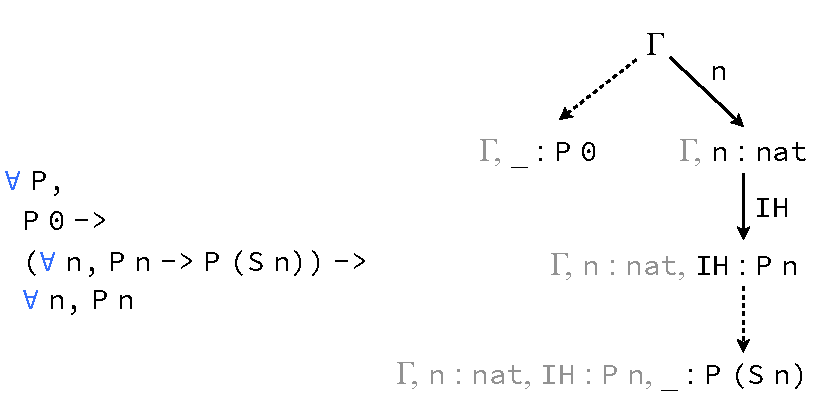
\includegraphics[scale=0.55]{repair/nat_ind}
\end{center}
\caption{The type of (left) and tree for (right) the induction principle \lstinline{nat_ind}. The solid edges represent hypotheses, and the dotted edges represent the proof obligations for each case in an inductive proof.}
\label{fig:cattree}
\end{figure}

\subsubsection{Patch Specialization} Specialization (\lstinline{specialize.ml}) takes a patch candidate and some arguments,
all of which are Coq terms.
It applies the candidate to the arguments, then it $\beta\iota$-reduces~\cite{equality} the result using Coq's
\lstinline{Reduction.nf_betaiota} function. It is the job of the 
patch finding procedure to provide both the candidate and the arguments.

\subsubsection{Patch Abstraction} Abstraction (\lstinline{abstraction.ml}) takes a patch candidate, 
the goal type, and the function arguments or function to abstract.
It first generalizes the candidate, wrapping it inside of a lambda from the type of the term to abstract.
Then, it substitutes terms inside the body with the abstract term.
It continues to do this until there is nothing left to abstract, then filters results by the goal type.
Consider, for example, abstracting this candidate by \lstinline{m}:

\begin{lstlisting}[language=coq]
    fun (H : n <= m) => le_plus_trans n m 1 H(@\vspace{-0.04cm}@)
    : n <= m -> n <= m + 1
\end{lstlisting}

The generalization step wraps this in a lambda from some \lstinline{nat}, the type of \lstinline{m}:

\begin{lstlisting}[language=coq]
    fun ((@\diff{n0}@) : nat) =>(@\vspace{-0.04cm}@)
      (fun (H : n <= m) => le_plus_trans n m 1 H)(@\vspace{-0.04cm}@)
    : (@\ltacforall@) (@\diff{n0}@), n <= m -> n <= m + 1
\end{lstlisting}

The substitution step replaces \lstinline{m} with \lstinline{n0}:

\begin{lstlisting}[language=coq]
    fun ((@\diff{n0}@) : nat) =>(@\vspace{-0.04cm}@)
      (fun (H : n <= (@\diff{n0}@)) => le_plus_trans n (@\diff{n0}@) 1 H)(@\vspace{-0.04cm}@)
    : (@\ltacforall@) (@\diff{n0}@), n <= (@\diff{n0}@) -> n <= (@\diff{n0}@) + 1
\end{lstlisting}

Abstraction uses a list of \textit{abstraction strategies} to determine what subterms
to substitute. In this case, the simplest strategy works: The tool
replaces all terms that are convertible to the concrete argument \lstinline{m} with the abstract argument
\lstinline{n0}, which produces a single candidate. Type-checking this candidate confirms that it is a patch.

In some cases, the simplest strategy is not sufficient, even when it is possible to abstract the term.
It may be possible to produce a patch only by abstracting \emph{some} of the subterms
convertible to the argument or function (we show an example of this in Section~\ref{sec:fail}),
or the term may not contain any subterms convertible to the argument or function at all.
We implement several strategies to account for this. The combinations strategy, for example,
tries all combinations of substituting only some of the convertible subterms with the abstract argument. 
The pattern-based strategy substitutes subterms that match a certain pattern
with a term that corresponds to that pattern.
% TODO also, in general, not always possible

It is the job of the patch finding procedure to provide the candidate and the terms to abstract.
In addition, each configuration includes a list of strategies.
The configuration for changes in conclusions, for example, starts with the simplest strategy,
and moves on to more complex strategies only if that strategy fails.
This design makes abstraction simple to extend with new strategies and simple to call with different strategies
for different classes of changes; we identify new strategies in Section~\ref{sec:fail}.
% TODO Link to eval here if you eval this

\subsubsection{Patch Inversion} Patch inversion (\lstinline{inverting.ml}) exploits symmetry to try to reverse the conclusions of a 
candidate patch.
%That is, given a patch with type \lstinline{H -> C -> C'}, inversion attempts to modify the term
%to produce an inverse patch of type \lstinline{H -> C' -> C}. 
It first factors the candidate using the factoring component, then calls the primitive inversion
function on each factor, then finally folds the resulting list in reverse.
The primitive inversion function exploits symmetry. 
For example, equality is symmetric, so the component can invert any application of \lstinline{eq_ind} or \lstinline{eq_ind_r}
(any rewrite). Indeed, \lstinline{eq_ind} and \lstinline{eq_ind_r} are inverses, and are related by symmetry:

\begin{lstlisting}[language=coq]
   (@\diff{eq\_ind\_r}@) A x P (H : P x) y (H0 : y = x) :=(@\vspace{-0.04cm}@)
     (@\diff{eq\_ind}@) x (fun y0 : A => P y0) H y ((@\diff{eq\_sym}@) H0)	
\end{lstlisting}

If inversion does not recognize that the type is symmetric, it
swaps subterms and type-checks the result to see if it is an inverse.
In the future, it may be possible to use this swapping functionality
in a reflexive application of the induction principle to infer
symmetry properties like \lstinline{eq_sym} for other types. The component can then use these properties 
to generate reverse induction principles like \lstinline{eq_ind_r}. 
We further detail inversion in Section~\ref{sec:fail}.
% TODO above is ripped from 7.1 since we got rid of that subsection

\subsubsection{Lemma Factoring} The lemma factoring component (\lstinline{factoring.ml}) searches within a term
for its factors. For example,
if the term composes two functions, it returns both factors:

\begin{lstlisting}[language=coq]
    t : (@\diff{X}@) -> (@\diff{Z}@)                (* term *)(@\vspace{-0.04cm}@)
   [f : (@\diff{X}@) -> (@\diff{Y}@); g : (@\diff{Y}@) -> (@\diff{Z}@)] (* factors *)
\end{lstlisting}

In this case, the component takes the composite term and \lstinline{X} as arguments.
It first searches as deep as possible for a term of type \lstinline{X -> Y} for some \lstinline{Y}.
If it finds such a term, then it recursively searches for a term with type \lstinline{Y -> Z}. 
It maintains all possible 
paths of factors along the way, and it discards any paths that cannot reach \lstinline{Z}.

The current implementation can handle paths
with more than two factors, but it fails when \lstinline{Y} depends on \lstinline{X}.
Other components may benefit from dependent factoring; we leave this to future work.

\subsection{Inside the Procedure}
\label{sec:algimpl}

The implementation (\lstinline{patcher.ml4}) of the procedure from Section~\ref{sec:composeintro} starts with a
preprocessing step which compiles the proof terms to trees (like the tree in Figure~\ref{fig:cattree}).
It then searches for candidates one step at a time, expanding the trees when necessary.

\lstset{language=ml4}
The \sysname prototype exposes the patch finding procedure to users through the Coq 
command \lstinline{Patch Proof}. \sysname automatically
infers which configuration to use for the procedure from the example change. For example, to
find a patch for the case study in Section~\ref{sec:compcert}, we
used this command:

\begin{lstlisting}[language=ml4]
 Patch Proof Old.unsigned_range unsigned_range as patch.
\end{lstlisting}

\sysname analyzed both versions of \lstinline{unsigned_range} and determined 
that a constructor of the \lstinline{int} type changed (Figure~\ref{fig:int}),
so it initialized the configuration for changes in constructors.
%When \sysname needs the type of an intermediate lemma to guide search (as in Section~\ref{sec:foundations}), the user can pass that information to the command:

%\begin{lstlisting}[language=ml4]
% Patch Proof ... cut by (fun args => lemma args). 
%\end{lstlisting}

%When \sysname needs extra guidance, as in the case study in Section~\ref{sec:}

% TODO cutting lemmas

Internally, \sysname represents configurations as sets of options,
which it passes to the procedure. The procedure uses these options to determine
how to compose components (for example, whether to abstract candidates) 
and how to customize components (for example, whether semantic differencing should look for an intermediate lemma).
To implement new configurations for different classes of changes, we simply tweak the options.


%We have already demonstrated four patch finding procedures. 

%We implement the procedure from Section~\ref{sec:composeintro} as follows:

%\begin{algorithm}
%\footnotesize
%\begin{algorithmic}[1]
%  Is it really necessary to say that an algorithm might do initialization?
%  \STATE Build trees for search
%  \STATE build trees for proofs
%  \REPEAT
%    \STATE \textit{diff} nodes for goals
%    \STATE \textit{diff} edges for candidates
%    \IF{there are candidates}
%      \STATE \textit{factor}, \textit{abstract}, \textit{specialize}, and/or \textit{invert} candidates
%      \IFRETURN{there are patches}{patches}
%    \ENDIF
%    \STATE expand trees
%  \UNTIL{trees are fully expanded}
%  \IF{yet to reverse search direction}
%    \STATE restart from (2) in the opposite direction
%    \STATE \textit{factor} and \textit{invert} candidates
%    \IFRETURN{there are patches}{patches}
%  \ENDIF
%  \RETURN failure
%\end{algorithmic}
%\caption{Common Procedure Implementation}
%\label{alg:patchingcommon}	
%\end{algorithm}

%;
%since \sysname does not modify the Coq type checker, it
%cannot produce an ill-typed term.

\subsection{Trusted Computing Base}
\label{sec:tcb}

A common concern for Coq plugins is an increase in the trusted computing base.
The Coq developers provide a safe plugin API in Coq 8.7 to address this~\cite{coq87news}.
Our prototype takes this into consideration:
While \sysname does not yet support Coq 8.7, it only calls the internal Coq functions that the 
developers plan to expose in the safe API~\cite{coqPR}.
Furthermore, Coq type-checks terms that plugins produce.
Since \sysname does not modify the type checker, it cannot produce an ill-typed term.



%\section{Testing Boundaries}
\label{sec:eval}

\begin{figure*}[ht]
\begin{minipage}{0.48\textwidth}
\begin{lstlisting}[language=coq]
fun n m p (H : n <= m) (H0 : m <= p) =>(@\vspace{-0.04cm}@)
  (@\diff{le\_S n p}@) (* ... proof of stronger lemma *)(@\vspace{-0.04cm}@)
: (@\ltacforall@) n m p, n <= m -> m <= p -> n <= (@\diff{S p}@)
\end{lstlisting}
\end{minipage}
\hfill
\begin{minipage}{0.48\textwidth}
\begin{lstlisting}[language=coq]
fun n m p (H : n <= m) (H0 : m <= p) =>(@\vspace{-0.04cm}@)
  (@\diff{le\_plus\_trans n p 1}@) (* ... proof of stronger lemma *)(@\vspace{-0.04cm}@)
: (@\ltacforall@) n m p, n <= m -> m <= p -> n <= (@\diff{p + 1}@)
\end{lstlisting}
\end{minipage}
\vspace{-.35cm}
\caption{Two proof terms \lstinline{old} (left) and \lstinline{new} (right) that contain the same proof of a stronger lemma.}
\label{fig:stronger}
\end{figure*}

\lstset{language=coq, aboveskip=3pt,belowskip=3pt}

In the case studies in Section~\ref{sec:case}, we showed how
the core components are useful for real scenarios.
In this section, we explore the boundary between what the \sysname prototype can and cannot handle.
It is precisely this boundary that informs us how to improve the implementations of the
core components.

To evaluate this boundary, we tested the core components of \sysname on a suite of 50 pairs of proofs (Section~\ref{sec:suite}).
We designed 11 of these pairs to succeed, then modified their proofs to produce the remaining 39 pairs
that try to stress the core functionality of the tool.
%28 of the 50 variants did not stress \sysname at all.
We learned the following from the pairs
that tested \sysname's limitations:

\begin{enumerate}
\item \textbf{The failed pairs drive improvements.} \\
\sysname failed on 17 of 50 pairs. These pairs tell us how to improve the core. (Section~\ref{sec:fail})
\item \textbf{The pairs unearth abstraction strategies.} \\
\sysname produced an exponential number of candidates in 5 of 50 pairs.
New abstraction strategies can dramatically reduce the number of candidates. (Section~\ref{sec:fail})
\item \textbf{\sysname was fast, and it can be faster.} \\
The slowest successful patch took \SI{48}{\ms}. The slowest failure took \SI{7}{\ms}.
Simple changes can make \sysname more efficient. (Section~\ref{sec:perf})
\end{enumerate}

\subsection{Patch Generation Suite}
\label{sec:suite}

We wrote a suite\footnote{\url{http://github.com/uwplse/PUMPKIN-PATCH/blob/cpp18/plugin/coq/Variants.v}} of 50 pairs of proofs.
We wrote these proofs ourselves since searching for proof patches is a new domain,
so there was no existing benchmark suite to work with.
We used the following methodology:
%We designed 11 pairs to succeed, then modified these pairs to produce the remaining 39 pairs
%that stress the functionalti
%We designed 11 pairs to succeed:

\begin{enumerate}
\item Choose theorems \lstinline{old} and \lstinline{new}
\item Write similar inductive proofs of \lstinline{old} and \lstinline{new}
\item Modify the proof of \lstinline{old} to produce more pairs
\item Search for patches from \lstinline{new} to \lstinline{old}
\item If possible, search for patches from \lstinline{old} to \lstinline{new}
\end{enumerate}

In total, we chose 11 pairs of theorems \lstinline{old} and \lstinline{new}, and we wrote
50 pairs of proofs of those theorems.

For example, one pair of theorems \lstinline{old} and \lstinline{new} was a 
simplification of the auxiliary lemmas
that we encountered in the case study in Section~\ref{sec:foundations}.
For the first proof of \lstinline{old}, we added a rewrite, like in the case study:

\begin{lstlisting}[language=coq]
    (@\diff{rewrite <- plus\_n\_O.}@) rewrite -> plus_comm.
\end{lstlisting}

For the second proof of \lstinline{old}, we commuted the rewrites:

\begin{lstlisting}[language=coq]
    rewrite -> plus_comm. (@\diff{rewrite <- plus\_n\_O.}@)
\end{lstlisting} 

We then searched for patches in both directions,
since the conclusions of \lstinline{old}
and \lstinline{new} were propositionally equal.

Our goal was to determine what changes to proofs stress the components
and how to use that information to drive improvements.
We focused on differences in conclusions, the most supported configuration.
%The procedure defaults to \lstinline{old} when it cannot find a patch; 
%we marked each pair a success if \sysname found a direct patch,
%and a failure if it returned the default.
Since \sysname operates over terms,
we removed redundant proof terms, even if they were produced by different tactics.
We controlled the first pair of proofs of each pair of theorems for features we had not yet implemented,
like nested induction, changes in hypotheses, and abstracting \lstinline{omega} terms.
These features sometimes showed up in later proofs (for example, after moving a rewrite);
we kept these proofs in the suite, since isolated changes to supported proofs that
introduce unsupported features can inform future improvements.	

\subsection{Three Challenges}
\label{sec:fail}

\sysname found patches for 33 of the 50 pairs. 28 of the 33 successes
did not stress \sysname at all: \sysname found the correct candidate immediately and was able to abstract it
in one try.
The pairs that \sysname failed to patch and the successful pairs that stressed abstraction
reveal key information about how to improve the core components.
We walk through three examples.
Future tools can use these as challenge problems to improve upon \sysname.

\paragraph{A Challenge for Differencing} For one pair of proofs of theorems 
with propositionally equal conclusions (Figure~\ref{fig:stronger}),
the differencing component failed to find candidates in either direction.
These proofs both contain the same proof of a stronger lemma;
\sysname found patches from this lemma to
both \lstinline{old} and \lstinline{new},
but it was unable to find a patch between \lstinline{old} and \lstinline{new}.
A patch may show up deep in the difference between \lstinline{le_plus_trans}
and \lstinline{le_S}, but even if we $\delta$-reduce (unfold the definition of~\cite{equality}) \lstinline{le_plus_trans}, this is not obvious:

\begin{lstlisting}
    le_plus_trans n m p (H : n <= m) :=(@\vspace{-0.04cm}@)
      (fun lemma : m <= m + p =>(@\vspace{-0.04cm}@)
        trans_contra_inv_impl_morphism(@\vspace{-0.04cm}@)
          PreOrder_Transitive(@\vspace{-0.04cm}@)
          (m + p)(@\vspace{-0.04cm}@)
          m(@\vspace{-0.04cm}@)
          lemma)(@\vspace{-0.04cm}@)
      (le_add_r m p)(@\vspace{-0.04cm}@)
      H
\end{lstlisting}

This points to two difficulties in finding patches: Knowing when to $\delta$-reduce terms 
is difficult; exploring the appropriate time for reduction
may produce patches for pairs that \sysname currently cannot patch.
Furthermore, finding patches is more challenging
when neither theorem has a conclusion that is as strong as possible.

\paragraph{A Challenge for Inversion} For one pair of proofs with propositionally equal conclusions,
\sysname found a patch in one direction, but failed to invert it:

\begin{lstlisting}[language=coq]
    fun n m p (_ : n <= m) (_ : m <= p) (H1 : n <= p) =>(@\vspace{-0.04cm}@)
      gt_le_S n (S p) (le_lt_n_Sm n p H1)(@\vspace{-0.04cm}@)
    : (@\ltacforall@) n m p, n <= m -> m <= p -> n <= p -> S n <= S p
\end{lstlisting}

The inversion component was unable to invert this term, even though an inverse does exist.
To invert this, the component needs to know to $\delta$-reduce \lstinline{gt_le_S}:

\begin{lstlisting}[language=coq]
  gt_le_S n m :=(@\vspace{-0.04cm}@)
    (fun (H : (@\ltacforall@) n0 m0, (@\diff{n0 < m0}@) -> (@\diff{S n0 <= m0}@)) => H n m) (@\vspace{-0.1cm}@)
    ...(@\vspace{-0.1cm}@)
  : (@\ltacforall@) n m, (@\diff{n < m}@) -> (@\diff{S n <= m}@)
\end{lstlisting}

It then needs to swap the hypothesis with the conclusion in \lstinline{H} to produce the inverse:

\begin{lstlisting}[language=coq]
  gt_le_S$\inv$ n m :=(@\vspace{-0.04cm}@)
    (fun (H : (@\ltacforall@) n0 m0, (@\diff{S n0 <= m0}@) -> (@\diff{n0 < m0}@)) => H n m)(@\vspace{-0.1cm}@)
    ...(@\vspace{-0.1cm}@)
   : (@\ltacforall@) n m, (@\diff{S n <= m}@) -> (@\diff{n < m}@)
\end{lstlisting}

Inversion currently swaps subterms when it is not
aware of any symmetry properties about the inductive type. However,
it does not know when to $\delta$-reduce function definitions. Furthermore, 
there are many possible subterms to swap;
for inversion to know to only swap the subterms of \lstinline{H}, it must have a better
understanding of the structure of the term. Both of these are ways to improve inversion.

%\begin{figure*}[ht]
%\begin{minipage}{0.48\textwidth}
%\begin{lstlisting}[language=coq]
%Theorem old: (@\ltacforall@) l1 l2 : list nat,
%  length (@\diff{(rev (l1 ++ l2))}@) =
%  (length (@\diff{(rev l1)})@) + (length (@\diff{(rev l2)}@)).
%\end{lstlisting}
%\end{minipage}
%\hfill
%\begin{minipage}{0.48\textwidth}
%\begin{lstlisting}[language=coq]
%Theorem new: (@\ltacforall@) l1 l2 : list nat,
%  length (@\diff{(l1 ++ l2)}@) =
%  (length (@\diff{l1}@)) + (length (@\diff{l2}@)).
%\end{lstlisting}
%\end{minipage}
%\vspace{-.2cm}
%\caption{Two theorems \lstinline{old} (left) and \lstinline{new} (right) for which \sysname found patches in both directions.}
%\label{fig:list}
%\end{figure*}

\paragraph{A Challenge for Abstraction} Abstraction produced an exponential number of candidates when abstracting a patch candidate with this type:

\begin{lstlisting}[language=coq]
    (@\ltacforall@) n n0,(@\vspace{-0.04cm}@)
      (fun m => n <= max m n0) n ->(@\vspace{-0.04cm}@)
      (fun m => n <= max n0 m) n
\end{lstlisting}

The goal was to abstract by \lstinline{n} and produce a patch with this type:

\begin{lstlisting}[language=coq]
    (@\ltacforall@) (@\diff{m0}@) n n0,(@\vspace{-0.04cm}@)
      n <= max (@\diff{m0}@) n0 ->(@\vspace{-0.04cm}@)
      n <= max n0 (@\diff{m0}@)
\end{lstlisting}

%search found the following applied patch, For 5 variants, \sysname found a patch, but only after producing an exponential number of abstract candidates.
%While this did not have a significant impact on time, these variants uncover natural ways to extend abstraction
%to produce fewer candidates.
%For example, for one pair of proof terms, search found an applied patch:

The difficulty was in determining which occurrences of \lstinline{n} to abstract.
The component needed to abstract only the highlighted occurrences:

\begin{lstlisting}
    fun n n0 (H0 : n <= max n0 (@\diff{n}@)) =>(@\vspace{-0.04cm}@)
      @eq_ind_r (@\vspace{-0.04cm}@)
        nat (@\vspace{-0.04cm}@)
        (max n0 (@\diff{n}@))(@\vspace{-0.04cm}@)
        (fun n1 => n <= n1)(@\vspace{-0.04cm}@)
        H0(@\vspace{-0.04cm}@)
        (max (@\diff{n}@) n0)(@\vspace{-0.04cm}@)
        (max_comm (@\diff{n}@) n0)
\end{lstlisting}

The simplest abstraction strategy failed, and a more
complex strategy 
%substituted all occurrences of \lstinline{n} in the body with the abstract \lstinline{m0}.
%While this term was well-typed, it did not have the goal type.
%The next strategy substituted all combinations of occurrences of \lstinline{n} with \lstinline{m0},
%which eventually found a patch---
succeeded only after producing exponentially many candidates.
While this did not have a significant impact on time,
this case gives rise to a new class of abstraction strategies:
semantics-aware abstraction.
In this case, we know from the type of the candidate
and the type of \lstinline{eq_ind_r} that these two hypothesis types 
are equivalent (similarly for the conclusion types):

%Using the type signature of \lstinline{eq_ind_r},
%we can determine an alternative (equivalent) type for the candidate:

%\begin{lstlisting}[language=coq]
%    (@\ltacforall@) n n0,
%      (fun n1 => n <= n1) (max n0 n) ->
%      (fun n1 => n <= n1) (max n n0)
%\end{lstlisting}

%A simple semantics-aware strategy is to make sure that if we abstract any subterm, 
%we also abstract terms that depend on that subterm.
%This will dramatically reduce the number of candidates, but at the same time it does
%not require any advanced reasoning.

\begin{lstlisting}
    (fun m => n <= max m n0) n(@\vspace{-0.04cm}@)
    (fun n1 => n <= n1) (max n0 n)
\end{lstlisting}

The tool can search recursively for patches to find two patches that bridge the two equivalent
types:

\begin{lstlisting}
    p1 := fun n => max n0 n(@\vspace{-0.04cm}@)
    p2 := fun n => max n n0
\end{lstlisting}

Then the candidate type is exactly this:

\begin{lstlisting}
    (@\ltacforall@) n n0,(@\vspace{-0.04cm}@)
      (fun n1 => n <= n1) (@\diff{(p2 n)}@) ->(@\vspace{-0.04cm}@)
      (fun n1 => n <= n1) (@\diff{(p1 n)}@)
\end{lstlisting}

Abstraction should thus abstract the highlighted subterms and the
terms that have types constrained by those subterms.
%It should not change \lstinline{(fun n1 => n <= n1)}.
This produces a patch in one candidate:

\begin{lstlisting}
    fun (@\diff{m0}@) n n0 (H0 : n <= max n0 (@\diff{m0}@)) =>(@\vspace{-0.04cm}@)
      @eq_ind_r (@\vspace{-0.04cm}@)
        nat (@\vspace{-0.04cm}@)
        (max n0 (@\diff{m0}@))           (* p1 (@\diff{m0}@) *)(@\vspace{-0.04cm}@)
        (fun n1 => n <= n1) (* P *)(@\vspace{-0.04cm}@)
        H0                    (* : P (p1 (@\diff{m0}@)) *)(@\vspace{-0.04cm}@)
        (max (@\diff{m0}@) n0)           (* p2 (@\diff{m0}@) *)(@\vspace{-0.04cm}@)
        (max_comm (@\diff{m0}@) n0)      (* : p1 (@\diff{m0}@) = p2 (@\diff{m0}@) *)
\end{lstlisting}

%This is a significant engineering effort, but it generalizes beyond this case.
This same strategy would find a patch for one of the pairs that \sysname failed to 
abstract. %This suggests that even if this strategy increases runtime,
%it 
This is a natural future direction for abstraction.

\subsection{Performance}
\label{sec:perf}

\sysname performed well for all pairs. The slowest success took \SI{48}{\ms}.\footnote{i7-4790K, at 4.00 GHz, 32 GB RAM}
When \sysname failed, it failed fast. The slowest failure took \SI{7}{\ms}.
While we find this promising, proof terms were small ($\le$ 67 LOC);
we leave evaluating performance on larger terms
to future work.

%When \sysname failed, it failed fast. The slowest failure took \SI{7}{\ms}.
%This was a case of nested induction, which we are yet to implement: \sysname interpreted the difference of parameters
%in the nested inductive case as significant and tried to abstract that candidate. This difference
%was not actually significant, so search failed.

% TODO double-check that that's true

\sysname was slowest %at finding patches 
when the patch showed up inverted in the difference of proofs,
since \sysname had to search twice, once in each direction.
A future procedure may %implement search in both directions at once,
%or may 
determine which direction to search first ahead of time; proof term size may be a simple heuristic for this.

%; we suspect this will impose a slight overhead in the easy
%direction, but reduce the overhead in the difficult direction. Alternatively, future procedures may determine


%first searches for a patch from \lstinline{old} to \lstinline{new}, and if that fails,
%only then does it search backwards for a patch from \lstinline{new} to \lstinline{old}. If it finds a 
%an inverted patch, it then attempts to invert it.
%This means that it searches twice, once in each direction, and then uses the lemma factoring and inversion components.

%For example, \sysname was able to patch two proofs of the theorems \lstinline{old} and \lstinline{new} in Figure~\ref{fig:list} in %both directions.
%However, \sysname was much faster in finding the patches from \lstinline{new} to \lstinline{old} than it
%was at finding patches from \lstinline{old} to \lstinline{new}: It took
%\SI{2}{\ms} to patch the first variant and \SI{10}{\ms} to patch the second variant, whereas in the opposite direction, it
%took \SI{4}{\ms} to patch the first variant and \SI{18}{\ms} to patch the second variant.

%It makes sense that \sysname was slower in searching from \lstinline{old} to \lstinline{new}: The current algorithm
%first searches for a patch from \lstinline{old} to \lstinline{new}, and if that fails,
%only then does it search backwards for a patch from \lstinline{new} to \lstinline{old}. If it finds a 
%an inverted patch, it then attempts to invert it.
%This means that it searches twice, once in each direction, and then uses the lemma factoring and inversion components.

%Future algorithms may implement search in both directions at once; we suspect this will impose a slight overhead in the easy
%direction, but reduce the overhead in the difficult direction. Alternatively, future algorithms may determine
%sswhich direction to search first ahead of time; proof term size may be a simple heuristic for this.







%\section{Conclusions \& Future Work}
\label{sec:future}

Our vision is a future of proof automation in ITP that 
adapts proofs to breaking changes. This will unify the spirit of ITP---collaboration
between the programmer and the tool---with the realities of modern proof engineering:
Verification projects are large, specifications evolve over time,
and dependencies change and break backward-compatibility. Too much of the burden
of change rests on the programmer; not enough rests on the tool.

We conclude with a discussion of improvements that can help bring this vision to life.
% We have already discussed some small changes 
These improvements are driven by our experiences using the \sysname prototype
and by conversations within the ITP community.

%\subsection{Improving Core Components} We have shown that the five core components are key to a good proof patching tool.
%With that in mind, our implementation is far from perfect. 
%Three components in particular that have natural extensions that will improve performance significantly:

%\paragraph{Semantic Search} Search is the most complex component, and so it is naturally the one
%with the most room for improvement. One difficulty in search is determining when to reduce terms;
%exploring this possibility will produce patches for scenarios that \sysname cannot yet handle.
%\sysname has trouble inferring the arguments for specialization for certain kinds of proofs, especially
%those that pass through intermediate lemmas; improving search to support these cases will make the tool
%simpler to use. \sysname cannot infer the most efficient direction to search first,
%and instead relies on the user to supply the most efficient direction; using a simple heuristic like proof term size
%may cut the runtime of \sysname in half for certain pairs of proofs.

%\paragraph{Patch Abstraction} The abstraction component supports different strategies, but none of the current
%strategies use type information to guide which terms to abstract. Extending abstraction with
%semantics-aware strategies will not only cut down on the number of candidates that abstraction produces,
%but will also succeed in some cases on which abstraction currently fails.

%\paragraph{Patch Inversion} The inversion algorithm is currently aware only of symmetry properties of the equality types;
%in all other cases, it defaults to swapping subterms. It may be possible to use the subterm swapping functionality
%to infer symmetry properties of types, much like \lstinline{eq_sym}: First, generate a trivial reflexive application
%of the induction principle for the type. Then, swap some terms in that term. Inversion can then use these symmetry properties 
%to generate reverse induction principles like \lstinline{eq_ind_r}. That way, inversion can be strategic 
%about swapping subterms, and it never has to specialize to a particular type like \lstinline{eq}.

%\subsection{Improving Change Support} 
%\label{sec:futurechange}

%The ideal tool should support diverse changes.
%In addition to the component improvements we have already discussed,
%we see three ways to improve support:

\paragraph{Supporting structural changes.} Coq programmers often
make structural changes. It is common, for example, to
add new hypotheses, constructors, or parameters to a type.
The ideal tool should find patches for
these changes. %These are common changes;
%supporting these changes will make \sysname more useful.
Existing work in proof reuse~\cite{Boite2004, Mulhern06proofweaving}
and type-directed diffing~\cite{Miraldo:2017:TDS:3122975.3122976} may help guide these improvements.

\paragraph{Exploring new components.} The core components of \sysname are critical to searching for patches
in Coq, but they may not be sufficient for the ideal tool. While we find the flexibility of these components promising thus far, in implementing new features, we may discover new components. For example, patches for certain structural changes
may be program transformations as opposed to terms;
supporting these patches may reveal new components.

\paragraph{Modeling diverse proof styles.} Coq programmers use diverse proof styles;
the ideal tool should support many different styles.
Proofs about decidable domains that apply the term \lstinline{dec_not_not}
pose difficulties for abstraction and inversion; the ideal tool should support these. 
\sysname has limited support for changes in hypotheses, fixpoints, constructors, 
pattern matching, and nested induction; the ideal tool should implement these features.

\paragraph{Improving user experience.} The ideal proof patching tool should
be natural for programmers to use. A future patching tool
can produce tactics from the patches it finds, that way programmers
can remove references to old specifications. A future patching tool can integrate 
with an IDE (such as Proof General~\cite{proofgeneral})
or continuous integration (CI) system (such as Travis~\cite{travis}) to suggest
patches at natural steps in the development process.

%The ideal tool should support this workflow. A future patch finding tool
%can produce tactics from the patches it finds, 
%or can integrate with an IDE to suggest patches to programmers as they make changes or update dependencies.
% TODO old references, Travis

\paragraph{Handling version updates.} Updating Coq versions is an ideal use case for finding proof patches:
When the client updates Coq, a tool can automatically search commits to the standard library or to \lstinline{coq-contribs}
for patches.
In this case, the example comes from the Coq developers, not from the library client---the 
client never has to look at the changes that the Coq developers make.
The ideal tool should fully support updates in Coq versions.
\sysname can patch certain changes in the standard library, but it 
does not yet search for those changes automatically and determine which configuration to use depending on
what has changed. Furthermore, as proof assistant versions change, so may the AST and the plugin interface.
To fully support version updates, the tool should support different language versions.

\paragraph{Isolating changes.} Programmers sometimes make multiple changes to a verification project in the same commit;
the ideal tool should break down large changes into small, isolated changes to find patches.
This will help in finding benchmarks, supporting library and version updates, and integrating
with CI systems. We may draw on work in change and dependency management~\cite{873647, Autexier:2010:CMH:1986659.1986663, Celik:2017:IRP:3155562.3155588} to identify changes, then use the factoring component
to break these changes into smaller parts.

\paragraph{Supporting other proof assistants.} Coq is just one of many proof assistants;
ideal tools should support different proof assistants. While
\sysname focuses on Coq, the underlying concepts extend to other proof assistants with constructive
logics (for example, Lean~\cite{lean} and Agda~\cite{agda}).
Proof assistants with non-constructive logics (for example, Isabelle/HOL~\cite{isabellehol})
may benefit from a different approach; this is similar to the problem of finding patches for proofs of decidable domains in Coq, 
since classical properties provably hold for decidable propositions~\cite{decidable}.

\paragraph{Applying patches.} The ideal tool should not only find patches, but also apply the
patches it finds automatically to fix broken proofs. 
In some cases, this may be as simple as adding the patches as hints to a hint database, so that proofs go through with no changes.
However, hint databases in Coq cannot support certain terms~\cite{hints}, and adding too many
hints may impede performance.
More generally, we can integrate \sysname with a transfer tactic~\cite{Huffman2013, zimmermann2015automatic},
which is a perfect fit: 
Transfer tactics automatically adapt proofs between isomorphic types and implications, but they do
not find these functions; \sysname finds these functions, but it does not apply them.







%\chapter{Related Work}

% TODO whatever else isn't here yet, and some of this might be factored out or partially factored out---all papers, including survey, plus generals

\section{Programs}

\subsection*{Program Refactoring} 

Refactoring~\cite{Mens:2004:SSR:972215.972286}.

\subsection*{Program Repair} 

% From PUMPKIN PATCH, unchanged

Adapting proofs to changes is essentially program repair
for dependently typed languages. 
Program repair tools for 
languages with non-dependent type 
systems~\cite{Pei:2014:APR:2731750.2731779, Long:2016:APG:2837614.2837617, Le:2017:SSS:3106237.3106309, Mechtaev:2016:ASM:2884781.2884807, Monperrus2015} 
may have applications in the context of a dependently typed language.
Similarly, our work may have applications within program repair in these languages:
Future applications of our approach may repurpose it to repair programs for functional languages.

\subsection*{Ornaments}

% From PUMPKIN PATCH, unchanged

Ornaments~\cite{Dagand17jfp, Williams:2014:OP:2633628.2633631}
separate the computational and logical components of a datatype, and may
make proofs more resilient to datatype changes.

\subsection*{Programming by Example}

% From PUMPKIN PATCH, unchanged

Our approach generalizes an example that the programmer provides.
This is similar to programming by example, a subfield of 
program synthesis~\cite{DBLP:journals/ftpl/GulwaniPS17}. 
This field addresses different challenges in different logics,
but may drive solutions to similar problems in a dependently typed language.

\subsection*{Differencing \& Incremental Computation}

% From PUMPKIN PATCH, unchanged

Existing work in differencing and incremental computation may help 
improve our semantic differencing component.
Type-directed diffing~\cite{Miraldo:2017:TDS:3122975.3122976}
finds differences in algebraic data types.
Semantics-based change impact analysis~\cite{Autexier:2010:SCI:1860559.1860580} models semantic differences
between documents.
Differential assertion checking~\cite{differential-assertion-checking-2} analyzes different
versions of a program for relative correctness with respect to a specification.
Incremental $\lambda$-calculus~\cite{Cai:2014:TCH:2594291.2594304} introduces a general model for program changes.
All of these may be useful for improving semantic differencing.

\section{Proofs}

\subsection*{Proof Reuse}

% From PUMPKIN PATCH, unchanged

Our approach reimagines the problem of proof reuse in the context of proof automation.
While we focus on changes that occur over time, traditional proof reuse techniques can help
improve our approach.
Existing work in proof reuse focuses on transferring proofs between isomorphisms,
either through extending the type system~\cite{Barthe:2001:TIP:646793.704711} or through an automatic method~\cite{Magaud2002}.
This is later generalized and implemented in Isabelle~\cite{Huffman2013} and Coq~\cite{ZimmermannH15, tabareau:hal-01559073};
later methods can also handle implications. 
%Transfer tactics apply these functions but do not infer them, while our approach
%infers these functions but does not apply them.
Integrating a transfer tactic with a proof patch finding tool will create an end-to-end
tool that can both find patches and apply them automatically.

Proof reuse for extended inductive types~\cite{Boite2004} adapts proof obligations
to structural changes in inductive types. Later work~\cite{Mulhern06proofweaving} proposes a method
to generate proofs for new constructors. These approaches may be useful when extending the differencing
component to handle structural changes. Existing work in theorem reuse and proof generalization~\cite{Felty1994, pons00, Johnsen2004} abstracts existing proofs for reusability, and may be useful
for improving the abstraction component.
Our work focuses on the components critical to searching for patches; these complementary approaches
can drive improvements to the components.

\subsection*{Proof Evolution}

% From PUMPKIN PATCH, unchanged

There is a small body of work on change and dependency management for verification,
both to evaluate impact of potential changes and maximize reuse~\cite{873647, Autexier:2010:CMH:1986659.1986663}
and to optimize build performance~\cite{Celik:2017:IRP:3155562.3155588}.
These approaches may help isolate changes, which is necessary to identify future benchmarks, integrate
with CI systems, and fully support version updates.

\subsection*{Proof Refactoring}

\subsection*{Proof Repair}

\subsection*{Proof Design}

% From PUMPKIN PATCH, unchanged:

Existing proof engineering work addresses brittleness
by planning for changes~\cite{proof-eng} and designing theorems and proofs that make maintenance less of an issue.
Design principles for specific domains (such as formal metatheory~\cite{Aydemir2008, Delaware2013POPL, Delaware2013ICFP})
can make verification more tractable. CertiKOS~\cite{certikos} introduces the idea of a deep specification to
ease verification of large systems.
These design principles and frameworks are complementary to our approach.
Even when programmers use informed design principles,
changes outside of the programmer's control can break proofs;
our approach addresses these changes.

\subsection*{Proof Automation}

% From PUMPKIN PATCH, unchanged:

We address a missed opportunity in proof automation for ITP: searching
for patches that can fix broken proofs.
This is complementary to existing automation techniques. Nonetheless, there is a wealth
of work in proof automation that makes proofs more resilient to change.
Powerful tactics like \lstinline{crush}~\cite{chlipala:cpdt} can make
proofs more resilient to changes. 
Hammers like Isabelle's sledgehammer~\cite{Blanchette2013} can make proofs agnostic to some low-level changes.
Recent work~\cite{coqhammer} paves the way for a hammer in Coq.
Even the most powerful tactics cannot address all changes;
our hope is to open more possibilities for automation.

Powerful project-specific tactics~\cite{chlipala:cpdt, Chlipala2013} can help prevent low-level maintenance tasks.
Writing these tactics requires good engineering~\cite{Gonthier2011} and domain-specific knowledge,
and these tactics still sometimes break in the face of change.
A future patching tool may be able to repair tactics; the debugging process
for adapting a tactic is not too dissimilar to providing an example to a tool.

Rippling~\cite{rippling} is a technique for automating inductive proofs that uses restricted rewrite rules to
guide the inductive hypothesis toward the conclusion; this may guide improvements to the
differencing, abstraction, and specialization components.
The abstraction and factoring components address specific classes of unification problems;
recent developments to higher-order unification~\cite{Miller:2012:PHL:2331097} may help
improve these components.
Lean~\cite{selsam:lean} introduces the first congruence closure algorithm for dependent type theory that
relies only on the Uniqueness of Identity Proofs (UIP) axiom. While UIP is not fundamental to Coq,
it is frequently assumed as an axiom; when it is, it may be tractable to use a similar algorithm to improve the tool.

GALILEO~\cite{bundyreasoning} repairs faulty physics theories
in the context of a classical higher-order logic (HOL); there is preliminary work extending this
style of repair to mathematical proofs. 
Knowledge-sharing methods~\cite{tgck-cicm14} can adapt some proofs across different representations of HOL.
These complementary approaches may guide extensions to support decidable domains and classical logics.

\subsection*{Transport}

\subsection*{Parametricity}

\subsection*{Refinement}



